\documentclass[11pt]{article}
\usepackage[a4paper,margin=1in]{geometry}
\usepackage{amsmath,amssymb,amsthm,mathtools}
\usepackage[expansion=false]{microtype}
\usepackage{graphicx,booktabs,array}
\usepackage[font=small,labelfont=bf]{caption}
\usepackage[dvipsnames]{xcolor}
\usepackage{enumitem}
\usepackage[hidelinks,pdfusetitle]{hyperref}
\usepackage[nameinlink,capitalise]{cleveref}
\setlist{nosep,leftmargin=1.5em}
\newtheorem{theorem}{Theorem}[section]
\newtheorem{lemma}[theorem]{Lemma}
\newtheorem{proposition}[theorem]{Proposition}
\newtheorem{corollary}[theorem]{Corollary}
\newtheorem{conjecture}{Conjecture}
\theoremstyle{definition}\newtheorem{definition}[theorem]{Definition}
\theoremstyle{remark}\newtheorem{remark}[theorem]{Remark}
\newcommand{\R}{\mathbb R}\newcommand{\C}{\mathbb C}\newcommand{\N}{\mathbb N}
\newcommand{\dd}{\,\mathrm d}\newcommand{\e}{\mathrm e}
\newcommand{\Num}{\mathrm{Num}}\newcommand{\Den}{\mathrm{Den}}
\renewcommand{\Re}{\operatorname{Re}}\renewcommand{\Im}{\operatorname{Im}}
\setlength{\parskip}{0.35em}
\AtBeginDocument{\sloppy}
\urlstyle{same}
\hypersetup{pdftitle={Pair Balance and the Riemann Zeros: The Signed Current, the Mirror and the Merge, and the Prime Two},pdfauthor={Abhijit Singh}}
\title{\textbf{Pair Balance and the Riemann Zeros}\\[4pt]
\large The Signed Current, the Mirror and the Merge, and the Prime Two}
\author{Abhijit Singh}
\date{25 September 2026}
\begin{document}
\maketitle
\begin{abstract}
Riemann's function $\Xi(z)=\xi(\frac12+iz)$ is the Fourier transform of a positive, even, doubly-exponentially decaying kernel $\Phi$, and the Riemann Hypothesis (RH) is equivalent to the positivity of the current $J=2\partial_y|\Xi(x+iy)|^2$ for $y>0$. In this paper we write $J$ as a signed phase-space average of the Wigner function $Q$ of $\Phi$, $J=\frac14\int Q(p,x)\,p\sinh(yp)\,dp$, and prove the following. $Q$ has the exact expansion $Q=8e^{p/2}\sum_N\tau_x(N)\mathcal K_x(2\pi Ne^p)$ in Macdonald functions, with $\tau_x(N)=N^{-ix}\sigma_{2ix}(N)$ and Mellin transform $8\,\xi(w+ix)\xi(w-ix)$. $Q(p,x)>0$ whenever $2\pi e^{|p|}\ge\max(\sqrt{2x^2+\frac12},20)$, so that all Wigner negativity at momentum $|x|\ge14.14$ lies in $|p|<\log(x/2\pi)+\frac12\log2+O(x^{-2})$. RH holds if and only if every even position moment of $Q$ is nonnegative at every momentum. $J>0$ except on the set $\mathcal U$ where $|x|>3\cdot10^{12}-\frac12$ and $0<y<\frac12-1/(5.573412\log(|x|+\frac12))$. The coefficients $\tau_x(N)$ obey Euler-product lower bounds where the prime phases $x\log\ell$ align or alternate. An Epstein zeta function with the functional equation and no Euler product has a kernel with an expansion and a tail theorem of the same form and a current that is negative near its zero off the line, so a proof that $J\ge0$ on $\mathcal U$ must use a property such as the Euler product. We state this remaining step as a conjecture equivalent to RH.

The Euler product is a merge. $\xi$ is the moment function of two merged copies of one random unit, $\mathbb E[Y^s]=2\xi(s)$; we show that one copy gives $s\pi^{-s/2}\Gamma(\frac s2)\eta(s)$, the completed alternating series of the prime two, whose zeros on $\Re s=1$ have no mirror partners, and that among $\nu$ merged copies the mirror $s\mapsto1-s$ holds only at $\nu=2$. Followed in $\nu$, the first zero moves from $1+2\pi i/\log2$ at $\nu=1$ to $\frac12+14.134725\,i$ at $\nu=2$, the only point of its path on the critical line. The Davenport--Heilbronn function, which has the mirror and not the merge, has four mirrored pairs of zeros off the line below height $200$, while all $114$ zeros of $L(s,\chi_{-3})$ there lie on it. In $\mathbb Z/3$ every pair $\{s,-s\}$ sits at $\frac13$ and $\frac23$, $L(0,\chi_{-3})=\frac13$, and the three-state spin whose Lee--Yang zeros lie at the thirds is the positive merge of two elementary pairs. RH is the balance of the parity of the number of prime factors to within $x^{1/2+\varepsilon}$, which we follow exactly to $10^8$ ($49{,}998{,}058$ integers of even length against $50{,}001{,}942$ of odd length). At $x=50$ the margin of the criterion near the line is carried by the Airy transition zone of the expansion, and among $36$ heights in $[2\times10^5,3.2\times10^6]$ the three smallest margins occur where the phases of the primes up to $13$ align. The proofs use the Fourier expansion of the Eisenstein series, Riccati bounds for Macdonald functions of imaginary order, moment estimates and the Lee--Yang theorem; the computations evaluate the expansion in arithmetic of up to $200$ significant digits.
\end{abstract}

\tableofcontents

\section{Introduction}\label{sec:intro}

The Riemann Hypothesis (RH) is the conjecture that every nontrivial zero of the Riemann zeta function has real part $\frac12$. Equivalently, the entire function $\xi(s)=\frac12s(s-1)\pi^{-s/2}\Gamma(\frac s2)\zeta(s)$, which satisfies $\xi(s)=\xi(1-s)$, has all its zeros on the critical line $\Re s=\frac12$, and $\Xi(z)=\xi(\frac12+iz)$, an even entire function that is real on $\R$, has only real zeros.

\paragraph{Criteria.} RH has many equivalent forms. Littlewood showed that it is equivalent to $M(x)=\sum_{n\le x}\mu(n)=O(x^{1/2+\varepsilon})$ for every $\varepsilon>0$ \cite{Littlewood}, and the same holds for the summatory Liouville function $L(x)=\sum_{n\le x}\lambda(n)$ \cite{Borwein}; the sharper statements $L(x)\le0$ and $|M(x)|<\sqrt x$ are false \cite{Haselgrove,Tanaka,OdlyzkoteRiele}. In the language of Laguerre-type inequalities, RH holds if and only if the generalised Laguerre inequalities for $\Xi$ hold at every real point \cite{Patrick}, \cite[Thm.~2.9]{CV}. Lagarias \cite{Lagarias}, crediting Hinkkanen, proved that RH is equivalent to $\Re\,\xi'/\xi(s)>0$ on $\Re s>\frac12$, and Sondow and Dumitrescu \cite{SD} that it is equivalent to $|\Xi(x+iy)|$ being nondecreasing in $y\ge0$ for every real $x$. De Bruijn \cite{deBruijn} and Newman \cite{Newman76} deformed $\Xi$ by the heat flow; the de Bruijn--Newman constant $\Lambda$ satisfies $\Lambda\ge0$ by the theorem of Rodgers and Tao \cite{RT} and $\Lambda\le0.2$ \cite[Cor.~2]{PT}, and RH is the statement $\Lambda=0$. Newman also read $\Xi$ as the partition function of a single spin, for which RH is a Lee--Yang property \cite{Newman74,Newman76,NewmanWu}.

\paragraph{Unconditional results.} RH has been verified for every zero with $0<\gamma\le3\cdot10^{12}$ \cite{PT}, and $\zeta(\sigma+it)\ne0$ for $\sigma\ge1-1/(5.573412\log|t|)$, $|t|\ge2$ \cite{MT}. Hardy proved that infinitely many zeros lie on the critical line, and Selberg that a positive proportion of them do \cite[Ch.~X]{Titchmarsh}. \Cref{tab:prop} lists the successive lower bounds for that proportion, which now exceeds two thirds.
\begin{table}[h]\centering\small
\begin{tabular}{@{}lll@{}}\toprule
Proportion of zeros on the critical line & Authors & Year\\\midrule
more than $\frac13$ & Levinson \cite{Levinson} & 1974\\
more than $\frac25$ & Conrey \cite{Conrey} & 1989\\
more than $\frac5{12}$ & Pratt, Robles, Zaharescu, Zeindler \cite{PRZZ} & 2020\\
at least $0.6725$, simple and on the line (preprint) & Alp\"oge, Furman \cite{AF} & 2026\\\bottomrule
\end{tabular}
\caption{Lower bounds for the proportion of the nontrivial zeros of $\zeta$, counted with multiplicity, that lie on the critical line.}\label{tab:prop}
\end{table}

\paragraph{Main results.} Riemann's kernel is
\begin{equation}\label{eq:Phi}
\Phi(u)=4\sum_{n\ge1}\bigl(2\pi^2n^4e^{9u/2}-3\pi n^2e^{5u/2}\bigr)e^{-\pi n^2e^{2u}},
\end{equation}
and
\[
\Xi(z)=\int_0^\infty\Phi(u)\cos(zu)\dd u=\frac12\int_\R\Phi(u)e^{izu}\dd u ;
\]
$\Phi$ is positive, even and doubly-exponentially decaying (\cref{sec:current}). We write $z=x+iy$, $H(x,y)=|\Xi(x+iy)|^2$ and $J(x,y)=2\,\partial_yH(x,y)$, the current, and
\[
Q(p,x)=\int_\R\Phi\Bigl(\frac{p+q}2\Bigr)\Phi\Bigl(\frac{p-q}2\Bigr)\cos(xq)\dd q ,
\]
so that $Q(p,x)=2\pi W_\Phi(\frac p2,x)$, where $W_\Phi$ is the Wigner function of $\Phi$ regarded as a wave function (\cref{sec:phase}). The main results of this paper are the following.

\begin{theorem}[the criterion in phase space]\label{mt:criterion}
For all $x,y\in\R$,
\[
H(x,y)=\frac18\int_\R Q(p,x)\cosh(yp)\dd p,\qquad J(x,y)=\frac14\int_\R Q(p,x)\,p\sinh(yp)\dd p ,
\]
and $\int_\R J(x,y)\dd x=4\pi\int_0^\infty\Phi(u)^2u\sinh(2yu)\dd u>0$ for every $y>0$. The following are equivalent:
\begin{enumerate}[label=(\alph*)]
\item RH;
\item $J(x,y)\ge0$ for all $x\in\R$ and all $y>0$;
\item $\int_\R Q(p,x)\,p^{2k}\dd p\ge0$ for all integers $k\ge0$ and all $x\in\R$.
\end{enumerate}
\end{theorem}

\begin{theorem}[exact expansion and tail positivity]\label{mt:tail}
For all real $p,x$, with $D=z\,d/dz$ and $\tau_x(N)=N^{-ix}\sigma_{2ix}(N)=\sum_{d\mid N}(d^2/N)^{ix}$,
\[
Q(p,x)=8e^{p/2}\sum_{N\ge1}\tau_x(N)\,\mathcal K_x(2\pi Ne^p),\qquad \mathcal K_x=\bigl((D+1)^2+x^2\bigr)\bigl(D^2+x^2\bigr)K_{ix},
\]
where $K_{ix}$ is the Macdonald function of imaginary order, and $\int_\R Q(p,x)e^{(w-\frac12)p}\dd p=8\,\xi(w+ix)\,\xi(w-ix)$ for all $w\in\C$. Moreover $Q(p,x)>0$ whenever $2\pi e^{|p|}\ge\max(\sqrt{2x^2+\frac12},20)$. Hence for $|x|\ge14.14$ every negative value of $Q(\cdot,x)$ lies at $|p|<\log(x/2\pi)+\frac12\log2+O(x^{-2})$, and $J(x,y)>0$ whenever $|x|\ge14.15$ and $y\ge5.24\sqrt{x^2+\frac14}$, and whenever $|x|<14.15$ and $y\ge64$.
\end{theorem}

\begin{theorem}[the current off $\mathcal U$]\label{mt:region}
For $y>0$,
\[
\frac JH=4\sum_w\frac{y-\Im w}{(x-\Re w)^2+(y-\Im w)^2},
\]
the sum over the zeros $w$ of $\Xi$ taken in conjugate pairs; a pair $w=\gamma\mp ib$ with $b>0$ contributes a term that is negative exactly on the open half-disk $(x-\gamma)^2+y^2<b^2$, and a real zero contributes a positive term. Moreover $J(x,y)>0$ if $|x|\le3\cdot10^{12}-\frac12$ or $y\ge\frac12-1/(5.573412\log(|x|+\frac12))$. Consequently RH holds if and only if $J\ge0$ on
\[
\mathcal U=\Bigl\{|x|>3\cdot10^{12}-\tfrac12,\ \ 0<y<\tfrac12-\frac1{5.573412\log(|x|+\frac12)}\Bigr\}.
\]
\end{theorem}

\begin{theorem}[the Euler product of the Wigner coefficients]\label{mt:euler}
$\tau_x$ is multiplicative, $\tau_x(\ell^k)=U_k(\cos(x\log\ell))$ for every prime $\ell$ and $k\ge0$, where $U_k$ is the Chebyshev polynomial of the second kind, and $\sum_N\tau_x(N)N^{-s}=\prod_\ell(1-2\cos(x\log\ell)\,\ell^{-s}+\ell^{-2s})^{-1}$ for $\Re s>1$. Let $\theta_\ell,\phi_\ell\in[0,\pi]$ be the distances of $x\log\ell$ from $0$ and from $\pi$ modulo $2\pi$, let $N=\prod_\ell\ell^{k_\ell}$, let $d(N)$ be its number of divisors and $\lambda(N)=(-1)^{\sum_\ell k_\ell}$. If $k_\ell(k_\ell+2)\theta_\ell^2\le6$ for every $\ell\mid N$, then
\[
\frac{\tau_x(N)}{d(N)}\ \ge\ \prod_{\ell\mid N}\Bigl(1-\frac{k_\ell(k_\ell+2)\,\theta_\ell^2}6\Bigr)\ \ge\ 0 ;
\]
if $k_\ell(k_\ell+2)\phi_\ell^2\le6$ for every $\ell\mid N$, the same bound holds for $\tau_x(N)/(\lambda(N)d(N))$ with $\phi_\ell$ in place of $\theta_\ell$.
\end{theorem}

\begin{theorem}[the mirror without the merge]\label{mt:epstein}
Let $Z_\epsilon(s)=\sum_{(m,n)\ne(0,0)}(2m^2+3n^2)^{-s}$ be the Epstein zeta function of the form $2m^2+3n^2$, which has no Euler product, and let $\xi_\epsilon(s)=s(s-1)(\sqrt6/\pi)^s\Gamma(s)Z_\epsilon(s)$. Then $\xi_\epsilon$ is entire, $\xi_\epsilon(s)=\xi_\epsilon(1-s)$, and $\xi_\epsilon(\frac12+iz)=\int_0^\infty\Phi_\epsilon(u)\cos(zu)\dd u$ with an explicit theta-series kernel $\Phi_\epsilon$ that is even, positive and $O(\exp(\frac52|u|-2\pi e^{|u|}/\sqrt6))$. Its Wigner function $Q_\epsilon$ has an exact expansion in Macdonald functions of order $2ix$ whose coefficients have the Dirichlet series $Z_\epsilon(s+ix)Z_\epsilon(s-ix)$, and $Q_\epsilon(p,x)>0$ whenever $4\pi e^{|p|/2}\ge\sqrt6\max(\sqrt{8x^2+\frac12},20)$. The current $J_\epsilon=2\partial_y|\xi_\epsilon(\frac12+i(x+iy))|^2$ takes negative values in the upper half-plane.
\end{theorem}

\begin{theorem}[the mirror holds only for the merged pair]\label{mt:nu}
For $\nu>0$ let $S_\nu=\frac2{\pi^2}\sum_{n\ge1}g_n/n^2$ with independent gamma variables $g_n$ of shape $\nu$ and scale $1$, the merge of $\nu$ copies of $S_1$, and let $M_\nu(s)=\mathbb E[(\pi S_\nu/2)^{s/2}]$, an entire function of $s$.
\begin{enumerate}[label=(\roman*)]
\item $M_2(s)=2\xi(s)$, and $\Phi(u)=e^{u/2}f_{\log Y}(u)$, where $f_{\log Y}$ is the density of $\log Y$ and $Y=\sqrt{\pi S_2/2}$ is the merged pair.
\item $M_1(s)=s\,\pi^{-s/2}\Gamma(\frac s2)\,\eta(s)$ with $\eta(s)=(1-2^{1-s})\zeta(s)$. It vanishes at $s=1+2\pi ik/\log2$ for every integer $k\ne0$, and not at the mirror images $-2\pi ik/\log2$ of these points.
\item For every $\nu>0$, $\log\bigl(M_\nu(1-2k)/M_\nu(2k)\bigr)=2k\log(2/\nu)+o(k)$ as $k\to\infty$ through the integers. Hence $M_\nu(s)=M_\nu(1-s)$ for all $s$ if and only if $\nu=2$.
\end{enumerate}
\end{theorem}

\begin{theorem}[pair balance and the prime two]\label{mt:prime2}
\begin{enumerate}[label=(\roman*)]
\item For $n\ge2$, $n$ is prime if and only if every map $x\mapsto ax$ with $a\ne0$ on $\mathbb Z/n\mathbb Z$ is bijective. The smallest rank of such a map is the smallest prime factor of $n$, which is $2$ for every even $n$.
\item RH holds if and only if $M(x)=O(x^{1/2+\varepsilon})$ for every $\varepsilon>0$, and if and only if $L(x)=O(x^{1/2+\varepsilon})$ for every $\varepsilon>0$.
\item For $\Re s>0$, $(1-2^{1-s})\zeta(s)=\sum_{k\ge1}\bigl[(2k-1)^{-s}-(2k)^{-s}\bigr]$, and $1-2^{1-s}$ vanishes only on $\Re s=1$. In $0<\Re s<1$ the zeros of $\zeta$ are therefore exactly the points at which this series of balanced pairs sums to zero.
\item The mirror $\mathsf R(s)=1-\bar s$ and conjugation generate a Klein four-group that acts on the nontrivial zeros, and RH holds if and only if every orbit has size $2$.
\end{enumerate}
\end{theorem}

\begin{theorem}[the thirds and the positive merge]\label{mt:thirds}
\begin{enumerate}[label=(\roman*)]
\item Let $a$ be the $q$-periodic sequence with $a_r=1$, $a_{r+g}=-1$ $(1\le r<r+g\le q)$ and $a_n=0$ at the other residues. Then $L(s,a)=\sum_na_nn^{-s}$ is entire and $L(0,a)=g/q$. In $\mathbb Z/3$ every pair $\{s,-s\}$ with $s\ne0$ is $\{1,2\}$, the odd functions vanishing at $0$ are the multiples of the completely multiplicative character $\chi_{-3}$, and $L(0,\chi_{-3})=\frac13$.
\item Two spins $\varsigma_1,\varsigma_2\in\{\pm\frac12\}$ merged with weight $e^{4\kappa\varsigma_1\varsigma_2}$, $\kappa\ge0$, have both Lee--Yang zeros on $|z|=1$. At $\kappa=\frac12\ln2$ the merged pair is the uniform three-state spin $\{-1,0,1\}$, whose zeros lie exactly at $\frac13$ and $\frac23$ of a turn, and every finite system of uniform three-state spins with couplings $\kappa_{jk}\ge0$ has all its Lee--Yang zeros on $|z|=1$.
\end{enumerate}
\end{theorem}

\Cref{mt:criterion} combines \cref{prop:HJ,prop:pairformula} with \cref{thm:moments}; \cref{mt:tail} combines \cref{thm:macdonald,thm:mellin,thm:tail} with \cref{prop:operator} and \cref{cor:calib}; \cref{mt:region} is \cref{prop:pairformula,prop:region}; \cref{mt:euler} is \cref{thm:euler}; \cref{mt:epstein} combines \cref{lem:epkernel} with \cref{thm:epstein} and the zeros of Davenport and Heilbronn (\cref{sec:epstein}); \cref{mt:nu} combines \cref{prop:bpy} with \cref{rem:eta}, \cref{cor:two} and \cref{prop:onlytwo}; \cref{mt:prime2} combines \cref{prop:field,prop:RH} with \cref{sec:eta}; and \cref{mt:thirds} is \cref{prop:cycle,prop:three,prop:spin}.

\paragraph{Relation to prior work.} Several ingredients are classical and are credited where they appear. The equivalence of (a) and (b) in \cref{mt:criterion} is the criterion of Sondow and Dumitrescu and of Lagarias \cite{SD,Lagarias}, and that of (a) and (c) is due, in the language of Laguerre inequalities, to Patrick and to Csordas and Varga \cite{Patrick,CV}; the expansion and the Mellin duality in \cref{mt:tail} are the Fourier expansion of the Eisenstein series and Hecke's integral \cite{Iwaniec}; the local factors in \cref{mt:euler} are classical; \cref{mt:prime2}(ii) is Littlewood's theorem and its parity form \cite{Littlewood,Borwein}; $M_2=2\xi$ in \cref{mt:nu}(i) is due to Biane, Pitman and Yor \cite{BPY}; the circle statements of \cref{mt:thirds}(ii) rest on the Lee--Yang theorem \cite{LeeYang,Griffiths69}; the Davenport--Heilbronn function is that of \cite{DH}, with the zeros located by Spira \cite{Spira}; and the zeros of $Z_\epsilon$ off the line are due to Davenport and Heilbronn \cite{DH}. New here, to our knowledge, are the phase-space formulation, the tail theorem with its explicit constants and its calibration, the bounds of \cref{mt:euler}, the self-contained proof of (a)$\Leftrightarrow$(c), the Epstein kernel as a limit on kernel-only arguments, the single-copy identity with $\eta$, the uniqueness of the mirror at $\nu=2$, the exact thirds, and the computations below.

\paragraph{Main computations.} The computations of this paper, by the methods of \cref{sec:methods}, give the following.
\begin{enumerate}[label=(\arabic*)]
\item The exact parity record to $10^8$: $49{,}998{,}058$ integers of even length against $50{,}001{,}942$ of odd length, and $|L(x)|/\sqrt x\le1.3583$ on $[10^4,10^8]$ (\cref{sec:balance}).
\item Followed in $\nu$, the first zero of $M_\nu$ moves from $1+2\pi i/\log2$ at $\nu=1$ to $\frac12+14.134725\,i$ at $\nu=2$, the only point of its path within $10^{-6}$ of the critical line (\cref{sec:xi}).
\item The Davenport--Heilbronn function, which has the mirror and not the merge, has eight zeros off the line with $0.5<t<200$, Spira's four mirrored pairs, while all $114$ zeros of $L(s,\chi_{-3})$ and all $122$ zeros of $L(s,\chi_{-4})$ in that range lie on it (\cref{sec:mirror,sec:merge}).
\item The Epstein function $Z_\epsilon$ has the zero $s_0=1.15958745297694888+9.45225081186590043\,i$, and $J_\epsilon(\Im s_0,y)$ changes sign at $y=\Re s_0-\frac12=0.6596$ (\cref{sec:epstein}).
\item At $x=50$ the margin $\Delta=1-A/G$ of the criterion near the line is carried by the Airy transition zone of the expansion (\cref{sec:ledger}).
\item Among $36$ heights in $[2\times10^5,3.2\times10^6]$, the three smallest margins at each of $y=0.05,0.1,0.3$ occur at the three heights where the phases $t\log\ell$, $\ell\le13$, align best (\cref{sec:heights}).
\end{enumerate}

\paragraph{The remaining step.} By \cref{mt:criterion,mt:region}, RH is equivalent to the positivity of the current on $\mathcal U$. We state this remaining step as a conjecture.
\begin{conjecture}\label{conj:target}
For every $x$ with $|x|>3\cdot10^{12}-\frac12$ and every $0<y<\frac12-1/(5.573412\log(|x|+\frac12))$,
\[
\int_\R Q(p,x)\,p\sinh(yp)\dd p>0 .
\]
\end{conjecture}
Conjecture~\ref{conj:target} is equivalent to RH. If RH holds, every term of the pair formula in \cref{mt:region} is positive and $H>0$ for $y>0$, so $J>0$; conversely, the conjecture and \cref{mt:region} give $J\ge0$ for all $y>0$, which is RH by \cref{mt:criterion}. By \cref{mt:epstein}, a proof must use a property that $\zeta$ has and $Z_\epsilon$ lacks; the one this paper isolates is the merge, the Euler product. \Cref{sec:target} collects five further equivalent forms proved in the paper and locates the step.

\paragraph{Methods of proof.} The phase-space identities follow from the substitution $p=u+v$, $q=u-v$ in $|\Xi|^2=\frac14\iint\Phi(u)\Phi(v)e^{izu-i\bar zv}\dd u\dd v$: the product of two copies of the kernel, rotated by $45^\circ$, is the Wigner function. Inserting the theta series for both copies and integrating over $q$ term by term turns each pair $(m,n)$ into a Macdonald function of argument $2\pi mne^p$, and the coefficient $\tau_x(N)$ collects the pairs with $mn=N$. The fourth-order operator that produces $\mathcal K_x$ from $K_{ix}$ is exactly the one that, under the Mellin transform, supplies the completing factors $s(s-1)$; this gives the duality with $\xi(w+ix)\xi(w-ix)$ and, at $w=\frac12+y$, the formulas for $H$ and $J$. For tail positivity, $\sqrt z\,K_{ix}(z)$ satisfies a Schr\"odinger equation whose potential $1-(x^2+\frac14)/z^2$ is nonnegative beyond the turning point; Riccati comparison then bounds $-K_{ix}'/K_{ix}$ and the decay of $K_{ix}(Nz)$ in $N$, so that for $2\pi e^{|p|}\ge\sqrt{2x^2+\frac12}$ the term $N=1$ exceeds the sum of all others by a factor above $10^4$. The unconditional region comes from the pair formula for $J/H$ together with the verification to height $3\cdot10^{12}$ and the zero-free region. The Euler-product bounds use $\tau_x(\ell^k)=U_k(\cos(x\log\ell))$ and a second-order bound for the Chebyshev ratio. The Epstein function has a kernel built from its own theta function by the same differential operator, so the expansion and the tail theorem transfer with $2x$ in place of $x$; what it lacks is an Euler product for its coefficients. For $\nu$ merged copies, Stirling estimates of the positive and negative moments compare $M_\nu(2k)$ with $M_\nu(1-2k)$. The computations evaluate the expansion in decimal arithmetic of $40$ to $200$ significant digits, because the Macdonald functions of order $ix$ lose about $0.68x$ digits to cancellation (\cref{sec:methods}).

\paragraph{Organisation.} \Cref{sec:zero,sec:balance,sec:eta} treat the pair and the prime two (\cref{mt:prime2}); \cref{sec:thirds,sec:horizon,sec:mirror,sec:merge,sec:xi} the triad, the horizon, the mirror and the merge (\cref{mt:thirds,mt:nu}); \cref{sec:current,sec:phase,sec:expansion,sec:mellin,sec:euler,sec:positive,sec:epstein} the signed current (\cref{mt:criterion,mt:tail,mt:region,mt:euler,mt:epstein}); and \cref{sec:ledger,sec:heights} measure where its margin lives. \Cref{sec:target} discusses the remaining step, \cref{sec:methods} gives the methods of computation, and \cref{sec:concl} concludes.

\paragraph{Notation.} $\Xi$ is an even entire function, real on $\R$, whose zeros are $z=\gamma-ib$ for the nontrivial zeros $\rho=\frac12+b+i\gamma$ of $\zeta$. The kernel \eqref{eq:Phi} is twice the kernel of \cite[(2.16.1)]{Titchmarsh}, whose representation reads $\Xi(t)=2\int_0^\infty\Phi_{\mathrm T}(u)\cos(ut)\dd u$.

\emph{The mirror.} $\iota(s)=1-s$ is the involution of the functional equation $\xi(s)=\xi(1-s)$, $s\mapsto\bar s$ is conjugation, and their composition $\mathsf R(s)=1-\bar s$ is the reflection in the critical line, which is its fixed set; we call $\mathsf R$ the mirror. With the identity they form the Klein group $V_4=\{\mathrm{id},\ \iota,\ s\mapsto\bar s,\ \mathsf R\}$. In the variable $z$, $\iota$ is $z\mapsto-z$, conjugation is $z\mapsto-\bar z$, and $\mathsf R$ is $z\mapsto\bar z$, that is $y\mapsto-y$; $H$ is even in $y$, which is the mirror, and the Wigner function $Q$ is even in $p$.

\emph{The merge.} Two units merge when their weights multiply: for arithmetic functions, $a(mn)=a(m)a(n)$, equivalently an Euler product; for independent random variables, the sum $X\oplus X'$ of independent copies, whose Laplace transforms multiply; for spins, the coupling $e^{\kappa\,\sigma\sigma'}$, a \emph{positive merge} when $\kappa\ge0$.

\emph{Arithmetic.} Primes are written $\ell$ (the letter $p$ is the Wigner position). $d(N)$ is the number of divisors, $\sigma_{2ix}(N)=\sum_{d\mid N}d^{2ix}$, $\Omega(n)$ and $\omega(n)$ are the numbers of prime factors with and without multiplicity, $\lambda(n)=(-1)^{\Omega(n)}$ is the Liouville function, $\mu$ the M\"obius function, $\Lambda$ the von Mangoldt function, $\delta(n)=[n=1]$, $M(x)=\sum_{n\le x}\mu(n)$ and $L(x)=\sum_{n\le x}\lambda(n)$. $N$ is \emph{$13$-smooth} if all its prime factors are at most $13$. $\|\cdot\|$ is the distance to the nearest integer, and heights on the critical line are written $t$.

\section{Zero is a pair, and the prime two}\label{sec:zero}

In a ring the additive identity $0$ and the multiplicative identity $1$ are tied together by distributivity. From $s\cdot0=s\cdot(0+0)=s\cdot0+s\cdot0$ follows $s\cdot0=0$, and from $s+(-1)s=s(1+(-1))=s\cdot0=0$ follows $(-1)s=-s$. Hence
\begin{equation}\label{eq:zero}
0=s+(-s)=s\,\bigl(1+(-1)\bigr),\qquad s=s\cdot1+0 .
\end{equation}
Every zero is a multiple of one pair-sum, $1+(-1)$, and every element is the image of the identity $1$ under multiplication by itself, displaced by the other identity, $0$. A system is degenerate exactly when its two identities coincide: if $0=1$ then $s=s\cdot1=s\cdot0=0$ for every $s$, and the system has one element. A system's first task is therefore to keep $0$ and $1$ apart.

\paragraph{Count, value and the prime two.} The integers modulo $n$ make the distinction between a \emph{count} and a \emph{value} precise. The count $n$ is the number of elements; as a value, $n=1+1+\cdots+1$ ($n$ terms) equals $0$. The smallest $n\ge1$ with $n\cdot1=0$ is the characteristic, and the characteristic is $0$ if no such $n$ exists, as for $\mathbb Z$.

\begin{proposition}\label{prop:field}
For $n\ge2$ the following are equivalent: (a) $n$ is prime; (b) $\mathbb Z/n\mathbb Z$ is a field; (c) $0$ is not a product of nonzero elements (no zero divisors); (d) for every $a\ne0$ the multiplication map $x\mapsto ax$ on $\mathbb Z/n\mathbb Z$ has full image, of size $n$ (full rank). For $n=1$ the system is degenerate ($0=1$). In any system with $1\ne0$ and without zero divisors, the characteristic is $0$ or a prime.
\end{proposition}
\begin{proof}
Put $g=\gcd(a,n)$. Then $ax=ay$ in $\mathbb Z/n\mathbb Z$ iff $n\mid a(x-y)$ iff $(n/g)\mid(x-y)$, so the image of $x\mapsto ax$ has exactly $n/g$ elements. Hence (d) holds iff $\gcd(a,n)=1$ for all $0<a<n$, i.e.\ iff $n$ is prime, so (d)$\Leftrightarrow$(a). Full rank means $x\mapsto ax$ is a bijection, so some $x$ has $ax=1$ and $a$ is invertible, giving (d)$\Rightarrow$(b); (b)$\Rightarrow$(c) is immediate, since $ab=0$ with $a$ invertible gives $b=a^{-1}ab=0$; if $n=ab$ with $1<a,b<n$ then $a\cdot b=0$, so (c)$\Rightarrow$(a). If a system without zero divisors had characteristic $n=ab$ with $1<a,b<n$, then $(a\cdot1)(b\cdot1)=n\cdot1=0$ would force $a\cdot1=0$ or $b\cdot1=0$, contradicting minimality \cite{Lang}.
\end{proof}
\noindent\emph{Smallest rank.} The largest proper divisor of $n$ is $n/\ell$, where $\ell$ is the smallest prime factor of $n$. By the proof above, the smallest rank of a nonzero multiplier is therefore $\min_{0<a<n}n/\gcd(a,n)=\ell$, attained at $a=n/\ell$. It equals $n$ exactly when $n$ is prime, and it equals $2$ for every even composite $n$. Direct enumeration for $2\le n\le30$, of all products $ab$ with $0<a,b<n$ and of the image of every map $x\mapsto ax$, confirms that (a), (c) and (d) select the same ten values of $n$, the primes up to $29$; \cref{fig:bal} (right) shows the ratio $\ell/n$ for $2\le n\le60$.

\begin{remark}[why $2$ is the smallest prime]\label{rem:two}
The following facts describe, from three sides, the one fact that $2$ is the least integer greater than $1$ that is not a product of smaller ones.
\begin{enumerate}
\item In the multiplicative monoid $(\mathbb Z_{>0},\times)$ the number $1$ is the identity, the empty product, so it is not an atom; $2$ is the smallest element other than the identity, hence the smallest atom.
\item $\mathbb Z/1\mathbb Z$ is the degenerate system $0=1$; $\mathbb Z/2\mathbb Z=\{0,1\}$ is the smallest system in which zero and identity are different, and it is a field.
\item $2$ is the order of the sign group $\{1,-1\}$, the units of $\mathbb Z$, i.e.\ of the involution $s\mapsto-s$. In $\mathbb Z/2\mathbb Z$ this involution is trivial: $-1=1$, $s+s=0$, every element is its own pair. For every odd prime $\ell$ the involution $s\mapsto-s$ on $\mathbb Z/\ell\mathbb Z$ has exactly one fixed point, $0$: $s=-s$ means $2s=0$, and $2$ is invertible modulo $\ell$.
\end{enumerate}
\end{remark}
The prime $2$ is thus the prime of the pair itself: the count at which the two members of $\{1,-1\}$ become one, and \eqref{eq:zero} reads $0=1+1$. It reappears inside every other prime. The group $(\mathbb Z/\ell\mathbb Z)^\times$ is cyclic of even order $\ell-1$ \cite{Lang}, so it has exactly one subgroup of index $2$. That subgroup is the image of the squaring map $x\mapsto x^2$, whose kernel is $\{1,-1\}$. The Legendre symbol therefore splits the nonzero residues into two equal halves of $(\ell-1)/2$, squares and non-squares.

\paragraph{What a prime is.} Three equivalent descriptions, in the terms of \eqref{eq:zero}: an atom of multiplication, a number of multiplicative length one; a count $\ell$ at which the identity, added to itself, returns to zero in a system where zero arises only additively, as $s+(-s)$, and never as a product of nonzero elements; a count at which every nonzero multiplier is a symmetry, of full rank.

\section{The Dirichlet identity and the balance of parities}\label{sec:balance}

$(\mathbb Z_{>0},\times)$ is the free commutative monoid on the primes: $n=\prod\ell^{k_\ell}$ uniquely. Its \emph{length} (order) is $\Omega(n)=\sum k_\ell$ and its \emph{rank}, the number of distinct primes, is $\omega(n)$. The M\"obius function is $\mu(n)=(-1)^{\omega(n)}$ if $n$ is squarefree and $\mu(n)=0$ otherwise. Arithmetic functions form a ring under Dirichlet convolution $(f*g)(n)=\sum_{d\mid n}f(d)g(n/d)$, whose identity is $\delta$. The constant function $\mathbf1$ (whose Dirichlet series is $\zeta$) has the inverse $\mu$ (whose series is $1/\zeta$), and $\mathbf1*\mu=\delta$ reads as follows. For $n>1$ only the squarefree divisors of $n$ contribute; a squarefree divisor with $j$ prime factors has $\mu(d)=(-1)^j$, and there are $\binom{\omega(n)}{j}$ of them. Hence
\begin{equation}\label{eq:mob}
\sum_{d\mid n}\mu(d)=\sum_{j=0}^{\omega(n)}\binom{\omega(n)}{j}(-1)^j=\bigl(1+(-1)\bigr)^{\omega(n)}=\begin{cases}1,&\omega(n)=0\ (n=1),\\0,&\omega(n)\ge1.\end{cases}
\end{equation}
The squarefree divisors of $n$ form the Boolean lattice of subsets of its $\omega(n)$ primes, $(\mathbb Z/2\mathbb Z)^{\omega(n)}$, with $\mu(d)=(-1)^{\text{rank of }d}$. \Cref{eq:mob} is the defining recursion of the M\"obius function of that lattice, equivalently the vanishing of the reduced Euler characteristic of the simplex on $\omega(n)\ge1$ vertices \cite{Rota}. Every $n>1$ is a zero of the form $s+(-s)$ at the level of its divisors, and the identity $\delta$ is the one place, rank $0$, where the pair $1+(-1)$ is not summed.

\emph{Squarefree density.} Write $n=m^2k$ with $k$ squarefree; then $d^2\mid n$ iff $d\mid m$, and \eqref{eq:mob} gives $\mu^2(n)=\sum_{d^2\mid n}\mu(d)$. Summing over $n\le x$,
\[
\#\{n\le x:\mu(n)\ne0\}=\sum_{d\le\sqrt x}\mu(d)\Bigl\lfloor\frac x{d^2}\Bigr\rfloor=x\sum_{d\ge1}\frac{\mu(d)}{d^2}+O(\sqrt x)=\frac{6}{\pi^2}\,x+O(\sqrt x),
\]
because dropping the floors and the terms $d>\sqrt x$ costs $O(\sqrt x)$, $\sum_d\mu(d)d^{-2}=1/\zeta(2)$ and $\zeta(2)=\pi^2/6$. Up to $10^8$ there are $60{,}792{,}694$ squarefree integers, against $6\cdot10^8/\pi^2=60{,}792{,}710$.

\paragraph{Balance of parities.} The Liouville function $\lambda(n)=(-1)^{\Omega(n)}$ is the homomorphism from $(\mathbb Z_{>0},\times)$ to $\{1,-1\}\cong\mathbb Z/2\mathbb Z$ that sends every prime to $-1$: length modulo $2$. For $\Re s>1$ the Euler products give
\[
\sum_{n\ge1}\frac{\mu(n)}{n^s}=\prod_\ell\bigl(1-\ell^{-s}\bigr)=\frac1{\zeta(s)},\qquad \sum_{n\ge1}\frac{\lambda(n)}{n^s}=\prod_\ell\frac1{1+\ell^{-s}}=\prod_\ell\frac{1-\ell^{-s}}{1-\ell^{-2s}}=\frac{\zeta(2s)}{\zeta(s)} .
\]
The second product is $\zeta(2s)\cdot\zeta(s)^{-1}$, so $\lambda(n)=\sum_{d^2\mid n}\mu(n/d^2)$ and
\begin{equation}\label{eq:LM}
L(x)=\sum_{d\le\sqrt x}M\bigl(x/d^2\bigr).
\end{equation}
\begin{proposition}[Littlewood; the parity form]\label{prop:RH}
\begin{equation}\label{eq:RH}
\mathrm{RH}\iff M(x)=O\bigl(x^{1/2+\varepsilon}\bigr)\ \forall\varepsilon>0\iff L(x)=O\bigl(x^{1/2+\varepsilon}\bigr)\ \forall\varepsilon>0 .
\end{equation}
\end{proposition}
\begin{proof}
RH implies the bound for $M$: this is Littlewood's theorem \cite{Littlewood}, see \cite[\S14.25]{Titchmarsh}. The bound for $M$ implies the bound for $L$ by \eqref{eq:LM}: $|L(x)|\le C\sum_{d\le\sqrt x}(x/d^2)^{1/2+\varepsilon}\le Cx^{1/2+\varepsilon}\sum_{d\ge1}d^{-1-2\varepsilon}$. Finally, if $L(x)=O(x^{1/2+\varepsilon})$ for every $\varepsilon>0$, partial summation gives $\zeta(2s)/\zeta(s)=s\int_1^\infty L(x)x^{-s-1}\dd x$, and the integral converges and is analytic in $\Re s>\tfrac12$. There $\zeta(2s)$ is finite and nonzero, since $\Re 2s>1$ and the Euler product converges; so $\zeta$ has no zero with $\Re s>\tfrac12$, and by the functional equation none with $0<\Re s<\tfrac12$ either, which is RH. The same argument with $1/\zeta(s)=s\int_1^\infty M(x)x^{-s-1}\dd x$ shows directly that the bound for $M$ implies RH. Both equivalences are collected in \cite{Borwein}.
\end{proof}
In the language of \eqref{eq:zero}: RH is the statement that the two members of the sign pair, integers of even and odd length (or the M\"obius signs), balance to within the square root of the count, up to $x^{\varepsilon}$.

\paragraph{The record to $10^8$.} The values of $\mu(n)$ and $\lambda(n)$ for all $n\le10^8$ were computed by sieving: for each prime $\ell\le10^8$ (sieve of Eratosthenes), $\mu$ and $\lambda$ are multiplied by $-1$ at every multiple of $\ell$, $\mu$ is set to $0$ at every multiple of $\ell^2$, and $\lambda$ is multiplied by $-1$ once more at every multiple of each power $\ell^k$, $k\ge2$. Then $M$ and $L$ are the cumulative sums, in exact integer arithmetic. The values at powers of ten agree with the published values \cite{OEISM,OEISL}:
\begin{center}\small
\begin{tabular}{@{}lcccccccc@{}}\toprule
$x$ & $10$ & $10^2$ & $10^3$ & $10^4$ & $10^5$ & $10^6$ & $10^7$ & $10^8$\\\midrule
$M(x)$ & $-1$ & $1$ & $2$ & $-23$ & $-48$ & $212$ & $1037$ & $1928$\\
$L(x)$ & $0$ & $-2$ & $-14$ & $-94$ & $-288$ & $-530$ & $-842$ & $-3884$\\\bottomrule
\end{tabular}
\end{center}
Up to $10^8$ there are $49{,}998{,}058$ integers of even length and $50{,}001{,}942$ of odd length. On $[10^4,10^8]$, $|M(x)|/\sqrt x\le0.4630$ (attained at $x=24185$, where $M=-72$) and $|L(x)|/\sqrt x\le1.3583$ (at $x=12{,}897{,}104$, where $L=-4878$); $L(x)\le0$ for every $2\le x\le10^8$. Two exact sharpenings of the balance are false: $L(x)\le0$ fails (Haselgrove \cite{Haselgrove}), first at $x=906{,}150{,}257$ (Tanaka \cite{Tanaka}), and $|M(x)|<\sqrt x$ fails for some $x$ \cite{OdlyzkoteRiele}. The content of RH is the square-root scale up to $x^\varepsilon$ (\cref{fig:bal}, left).

\begin{figure}[t]\centering
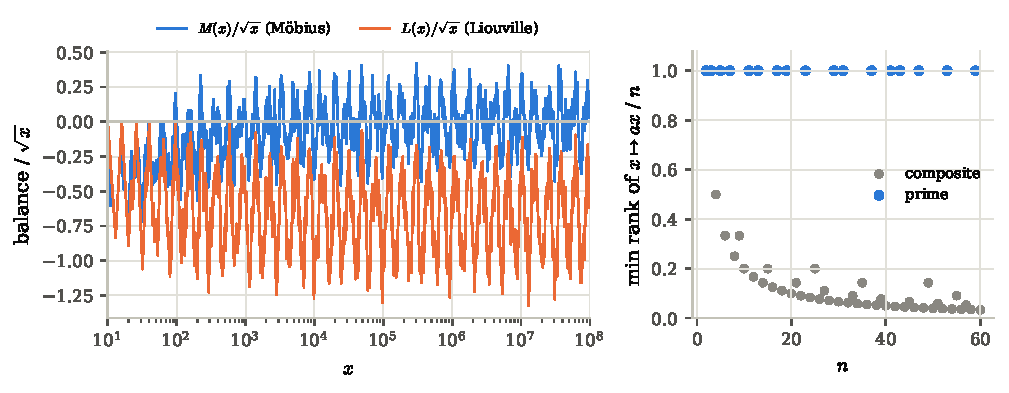
\includegraphics[width=\textwidth]{fig1_balance.pdf}
\caption{Left: the balance of the M\"obius signs, $M(x)/\sqrt x$, and of the parity of length, $L(x)/\sqrt x$, for $10\le x\le10^8$ (exact values on a logarithmic grid). RH is equivalent to both staying below $x^{\varepsilon}$ in this scale. Right: the smallest rank of a nonzero multiplication map on $\mathbb Z/n\mathbb Z$, as a fraction of $n$; it is $1$ exactly at the primes.}
\label{fig:bal}
\end{figure}

\section{The prime two inside \texorpdfstring{$\zeta$}{zeta}, and the mirror}\label{sec:eta}
Pairing each odd integer with the next even one gives the alternating series
\begin{equation}\label{eq:eta}
\eta(s)=\sum_{k\ge1}\Bigl[(2k-1)^{-s}-(2k)^{-s}\Bigr]=\bigl(1-2^{1-s}\bigr)\zeta(s)\qquad(\Re s>0).
\end{equation}
For $\Re s>1$, subtracting $2\cdot2^{-s}\zeta(s)=2\sum_k(2k)^{-s}$ from $\zeta(s)=\sum_nn^{-s}$ reverses the sign of every even term, which is \eqref{eq:eta}. Each pair is $(2k-1)^{-s}-(2k)^{-s}=s\int_{2k-1}^{2k}u^{-s-1}\dd u$, of modulus at most $|s|(2k-1)^{-\sigma-1}$ with $\sigma=\Re s$, so the paired series converges absolutely and locally uniformly in $\Re s>0$; both sides of \eqref{eq:eta} are analytic there, and the identity persists. The factor at the prime $2$ removes the pole: $1-2^{1-s}$ has a simple zero at $s=1$, and the pairs sum to $1-\tfrac12+\tfrac13-\cdots=\ln2$. The factor $1-2^{1-s}$ vanishes exactly when $(1-s)\ln2\in2\pi i\mathbb Z$, that is, only on the line $\Re s=1$. So in $0<\Re s<1$, $\eta$ and $\zeta$ have the same zeros, and a zero of $\zeta$ is a point where all these pairs balance: \eqref{eq:zero} with infinitely many terms.

\paragraph{The pairs balance at a zero.} Sum the first $K$ pairs of \eqref{eq:eta} and add the Euler--Boole tail correction $\tfrac12(2K+1)^{-s}$, the first term of the Euler--Boole expansion $\sum_{n>2K}(-1)^{n-1}n^{-s}=\tfrac12(2K+1)^{-s}+\tfrac s4(2K+1)^{-s-1}+O(|s|^3K^{-\sigma-3})$. With $K=10^6$ this reproduces $(1-2^{1-s})\zeta(s)$, with $\zeta$ from Euler--Maclaurin summation, to $9\times10^{-10}$ at $s=0.7+3i$, $0.5+10i$ and $2$, and $\ln2$ at $s=1$ to twelve digits. At $s=\frac12+i\gamma_1$, with $\gamma_1=14.134725141734693790$ \cite{Odlyzko}, the sum of $10^6$ pairs, whose absolute values total $8.8$, is $1.25\times10^{-9}$ in modulus. If $\eta(s)=0$, the corrected partial sum must equal minus the next Euler--Boole term, of modulus $\tfrac14|s|(2K+1)^{-3/2}$, up to $O(|s|^3K^{-7/2})$. It does: the computed moduli are $1.25\times10^{-6}$, $3.95\times10^{-8}$, $1.25\times10^{-9}$ for $K=10^4,10^5,10^6$, and $\tfrac14|s|(2K+1)^{-3/2}$ equals $1.25\times10^{-6}$, $3.95\times10^{-8}$, $1.25\times10^{-9}$. At $s=\frac12+17i$, which is not a zero, the same sum is $2.14$.

\paragraph{Each prime is a periodic pattern.} The factor $1-\ell^{-s}$ vanishes, and the Euler factor $(1-\ell^{-s})^{-1}$ has poles, exactly on the lattice $s=2\pi ik/\log\ell$, $k\in\mathbb Z$, strictly periodic with spacing $2\pi/\log\ell$: $9.0647$ ($\ell=2$), $5.7192$ ($3$), $3.9040$ ($5$), $3.2289$ ($7$), $2.6203$ ($11$), $2.4496$ ($13$). The factor $1-2^{1-s}$ of $\eta$ carries the lattice $1+2\pi ik/\log2$ onto the line $\Re s=1$: there $\eta$ vanishes (the pair sum with $K=10^6$ gives $|\eta|=5.7\times10^{-13}$ at $k=1$) although $\zeta(1+2\pi i/\log2)=1.3466+0.1099i\ne0$ (Euler--Maclaurin summation). The numbers $\log\ell$ are linearly independent over $\mathbb Q$: a relation $\sum_\ell q_\ell\log\ell=0$ with integers $q_\ell$ gives $\prod_\ell\ell^{q_\ell}=1$, and unique factorisation forces every $q_\ell=0$. Hence $2\pi ik/\log\ell=2\pi ik'/\log\ell'$ with $\ell\ne\ell'$ forces $k=k'=0$: no two of these lattices share a point other than $0$. By Kronecker's theorem \cite[Ch.~XXIII]{HardyWright}, the phases $t\log\ell$ modulo $2\pi$ of finitely many primes come arbitrarily close to any prescribed configuration. For $\sigma>1$, $\zeta(\sigma+it)=\prod_\ell(1-\ell^{-\sigma}e^{-it\log\ell})^{-1}$ is a product, uniformly convergent in $t$ (because $\sum_\ell\ell^{-\sigma}<\infty$), of factors each periodic in $t$ with period $2\pi/\log\ell$, and these periods are pairwise incommensurable. The zeros of $\zeta$ in the strip are zeros of the analytic continuation of this product of incommensurable periodic patterns, and they lie on none of the individual lattices. The heights at which many phases $t\log\ell$ align ($\equiv0$) or alternate ($\equiv\pi$) are those at which \cref{sec:heights} measures the smallest and largest margins of the criterion.

\paragraph{Order two acting on the zeros.} The functional equation $\xi=\xi\circ\iota$ and the reality $\xi(\bar s)=\overline{\xi(s)}$ make $V_4=\{\mathrm{id},\ \iota,\ s\mapsto\bar s,\ \mathsf R\}$, a group of order $4$, act on the zero set. The nontrivial zeros are not real: on $0<\sigma<1$ every pair $(2k-1)^{-\sigma}-(2k)^{-\sigma}$ is positive, so $\eta(\sigma)>0$, and since $1-2^{1-\sigma}\ne0$ there, $\zeta(\sigma)\ne0$. An orbit of a group of order $4$ has size $4/|\mathrm{stabiliser}|$. Conjugation fixes only real points, $\iota$ fixes only $s=\tfrac12$, and $\mathsf R$ fixes exactly the line $\Re s=\frac12$. A nontrivial zero $\rho$ is neither real nor equal to $\tfrac12$, so its orbit has size $4$, $\{\rho,1-\rho,\bar\rho,1-\bar\rho\}$, or size $2$, when $1-\rho=\bar\rho$, i.e.\ $\Re\rho=\frac12$. Hence
\begin{gather*}
\text{RH}\iff\text{every nontrivial zero is fixed by the mirror }\mathsf R\\
\iff\text{every orbit of }V_4\text{ on the nontrivial zeros has size }2 .
\end{gather*}
Zeros off the line come in quartets, and zeros on it in pairs. RH says that the zeros never use the full order of the group: each zero is its own mirror image, as every element of $\mathbb Z/2\mathbb Z$ is its own negative.

\section{The thirds are exact}\label{sec:thirds}
In the three-cycle the pair $s,-s$ sits at one third and two thirds of the system, measured from its zero, and merging the pair produces a representation with the same shares. Both statements are exact.

\begin{proposition}[a pair in a cycle]\label{prop:cycle}
Let $q\ge2$ and $1\le r<r+g\le q$. Let $a$ be the $q$-periodic sequence with $a_r=1$, $a_{r+g}=-1$ and $a_n=0$ at the other residues. Then $L(s,a)=\sum_{n\ge1}a_nn^{-s}$ is entire, and
\[
L(0,a)=\lim_{x\to1^-}\sum_{n\ge1}a_nx^n=\frac{r+g}{q}-\frac rq=\frac gq .
\]
The regularised value of the pair is the difference of the positions of $-s$ and $s$, measured in fractions of the cycle from its zero.
\end{proposition}
\begin{proof}
For $\Re s>1$, $L(s,a)=q^{-s}[\zeta(s,\tfrac rq)-\zeta(s,\tfrac{r+g}q)]$ with the Hurwitz zeta function $\zeta(s,\alpha)=\sum_{n\ge0}(n+\alpha)^{-s}$. Euler--Maclaurin summation of $f(x)=(x+\alpha)^{-s}$ gives
\[
\zeta(s,\alpha)=\frac{\alpha^{1-s}}{s-1}+\frac{\alpha^{-s}}2-s\int_0^\infty\Bigl(\{x\}-\tfrac12\Bigr)(x+\alpha)^{-s-1}\dd x ,
\]
and the integral converges for $\Re s>-1$ (integrate by parts once more against the bounded periodic antiderivative of $\{x\}-\frac12$). So $\zeta(s,\alpha)$ is meromorphic in $\Re s>-1$ with a single simple pole at $s=1$ of residue $1$, and $\zeta(0,\alpha)=-\alpha+\tfrac12$. The poles of the two Hurwitz zeta functions cancel, so $L(s,a)$ is entire (the same formula, iterated, continues it to all of $\C$), and $L(0,a)=(\tfrac12-\tfrac rq)-(\tfrac12-\tfrac{r+g}q)=\tfrac gq$. The Abel sum is $\sum_na_nx^n=(x^r-x^{r+g})/(1-x^q)\to g/q$ as $x\to1^-$.
\end{proof}
For all $286$ placements with $q\le12$, exact rational evaluation of $q^{-s}[\zeta(s,\frac rq)-\zeta(s,\frac{r+g}q)]$ at $s=0$ gives $g/q$; the Abel sum at $x=1-10^{-6}$ lies within $1.5\times10^{-6}$ of it, and the Euler--Maclaurin evaluation of the two Hurwitz zeta values within $1.6\times10^{-14}$. For $q=2$ the pair fills the cycle, the sequence is $(1,-1)$, and $\eta(0)=\tfrac12$: the elementary pair of \eqref{eq:eta} has the value one half.

\begin{proposition}[the three-cycle]\label{prop:three}
In $\mathbb Z/3\mathbb Z$:
\begin{enumerate}
\item For every $s\neq0$, $\{s,-s\}=\{1,2\}$. The pair always occupies the positions $\tfrac13$ and $\tfrac23$ of the cycle, and the two positions sum to $1$.
\item $s+(-s)=0$, while every product of elements of $\{1,2\}$ lies in $\{1,2\}$. Merging by multiplication returns the same two positions and never reaches the system zero, because $3$ is prime.
\item The functions on $\mathbb Z/3$ that are odd, $a(-n)=-a(n)$, and vanish at $0$ are exactly the multiples of $\chi_{-3}=(+1,-1,0)$, the sign of the position. This function is completely multiplicative, $\chi_{-3}(mn)=\chi_{-3}(m)\chi_{-3}(n)$, so $L(s,\chi_{-3})=\prod_\ell(1-\chi_{-3}(\ell)\ell^{-s})^{-1}$ for $\Re s>1$.
\item $L(0,\chi_{-3})=\tfrac23-\tfrac13=\tfrac13$. The reversed orientation, with $+1$ at position $\tfrac13$ and $-1$ at position $1$, has value $\tfrac23$.
\end{enumerate}
\end{proposition}
\begin{proof}
Parts (1) and (2) are the multiplication table of $\mathbb Z/3$. In part (3), oddness forces $a(2)=-a(1)$ and $a(0)=0$, and multiplicativity follows from (2). Part (4) is \cref{prop:cycle} with $q=3$.
\end{proof}

The same uniqueness holds for $q=4$, where the only such function is $\chi_{-4}=(1,0,-1,0)$. For $q\ge5$ the odd functions vanishing at $0$ form a space of dimension $\lfloor (q-1)/2\rfloor\ge2$: the values $a(1),\dots,a(\lfloor (q-1)/2\rfloor)$ are free, oddness fixes $a(q-n)=-a(n)$, and for even $q$ it forces $a(q/2)=-a(q/2)=0$. That space contains non-multiplicative members, and one of them is the Davenport--Heilbronn function of \cref{sec:mirror}. So in the three-cycle the pair and its merge come together: every balanced pair there merges. From the five-cycle on there are balanced pairs that do not.

\section{Three exact horizons}\label{sec:horizon}
The balance asserted by RH is a balance of opposites on either side of a horizon. The horizon has three exact forms.

\paragraph{The mirror of the functional equation.} Let $\theta(t)=\sum_{n\in\mathbb Z}e^{-\pi n^2t}$, which satisfies $\theta(1/t)=\sqrt t\,\theta(t)$. In Riemann's Mellin integral for $\xi$ the involution $t\mapsto1/t$ becomes $\iota$. The self-dual point $t=1$ becomes the critical line, and conjugation adds $s\mapsto\bar s$. The zeros are therefore mirrored across $\Re s=\tfrac12$: a zero at $\sigma+it$ has the partner $\mathsf R(\sigma+it)=1-\sigma+it$.

\paragraph{The Lee--Yang circle.} Regard $\frac12\Phi(u)\dd u$ as the (unnormalised) distribution of a spin $u$. Its partition function in a field $h$ is $Z_1(h)=\frac12\int_\R\Phi(u)e^{hu}\dd u=\Xi(-ih)$. RH says that $Z_1$ vanishes only for imaginary $h$, that is, only on the circle $|e^h|=1$. That circle separates the regions of positive and negative magnetisation, a horizon between opposite phases \cite{LeeYang,Newman74,NewmanWu}. We call this spin the Riemann spin.

\paragraph{A physical horizon.} Seen from one side of a Rindler horizon, the Minkowski vacuum is thermal at temperature $a/2\pi$. Each mode is paired with a partner on the other side, and the one-sided occupation is Bose--Einstein for bosons and Fermi--Dirac for fermions (four spacetime dimensions) \cite{Unruh,Takagi}. In the variable $x=2\pi\omega/a$, Riemann's own starting integrals are the Mellin transforms of these occupations:
\begin{equation}\label{eq:planck}
\Gamma(s)\zeta(s)=\int_0^\infty\frac{x^{s-1}}{e^x-1}\dd x,\qquad \Gamma(s)\eta(s)=\int_0^\infty\frac{x^{s-1}}{e^x+1}\dd x .
\end{equation}
Both follow by expanding $1/(e^x\mp1)=\sum_{n\ge1}(\pm1)^{n-1}e^{-nx}$ and integrating term by term with $\int_0^\infty x^{s-1}e^{-nx}\dd x=\Gamma(s)n^{-s}$ (for $\Re s>1$ and $\Re s>0$ respectively). The mode and its partner split the identity: with $n_{\mathrm B}(x)=1/(e^x-1)$ and $n_{\mathrm F}(x)=1/(e^x+1)$, $n_{\mathrm B}(x)+n_{\mathrm B}(-x)=\frac1{e^x-1}-\frac{e^x}{e^x-1}=-1$ for bosons and $n_{\mathrm F}(x)+n_{\mathrm F}(-x)=\frac1{e^x+1}+\frac{e^x}{e^x+1}=1$ for fermions. Both integrals in \eqref{eq:planck}, evaluated by adaptive quadrature at $s=2.5$ and $s=3+4i$, agree with $\Gamma(s)\zeta(s)$ and $\Gamma(s)\eta(s)$ to a relative $4\times10^{-15}$. The fermionic integral is the Mellin transform of the balanced pairs of \eqref{eq:eta}.

Three constructions attach the zeros to a dilation generator and a horizon:
\begin{itemize}
\item the Berry--Keating dilation Hamiltonian $xp$, whose semiclassical counting of states reproduces the smooth part of the counting function of the zeros \cite{BerryKeating};
\item a Dirac fermion in Rindler spacetime with mirrors placed by the primes \cite{Sierra};
\item gauging CPT at the black-hole horizon, which discretises the dilation spectrum into a set that corresponds to the zeros of $\zeta$ and of $L(s,\chi_{-4})$ \cite{BGP}; the latter is the four-cycle character of \cref{sec:thirds}.
\end{itemize}

\section{The mirror makes the opposites; the merge makes them meet}\label{sec:mirror}
\begin{proposition}\label{prop:mirror}
Let $F$ be meromorphic with $F=F\circ\iota$ and $F(\bar s)=\overline{F(s)}$. Then the zeros of $F$ come in sets $\{\rho,\bar\rho,1-\rho,1-\bar\rho\}$. An off-line zero at $\sigma+it$ has its mirror $\mathsf R(\sigma+it)=1-\sigma+it$. The two shares sum to one, and the product of the pair's sizes in an explicit formula is $|x^{\rho}|\,|x^{1-\bar\rho}|=x$ for every $\sigma$.
\end{proposition}
\begin{proof}
If $F(\rho)=0$ then $F(1-\rho)=F(\rho)=0$ and $F(\bar\rho)=\overline{F(\rho)}=0$, hence also $F(1-\bar\rho)=0$. For $\rho=\sigma+it$, $|x^\rho|\,|x^{1-\bar\rho}|=x^\sigma x^{1-\sigma}=x$.
\end{proof}
The mirror produces the opposites, and conservation fixes their total. Which $\sigma$ the pair takes is decided by the merge. The following function, which has the mirror but not the merge, shows that the merge clause carries the weight.

\paragraph{The Davenport--Heilbronn function.} Let $\vartheta\in(0,\frac\pi2)$ be defined by $\tan\vartheta=(\sqrt{10-2\sqrt5}-2)/(\sqrt5-1)=0.284079\ldots$ and
\[
f(s)=\sum_{n\ge1}a(n)n^{-s},\qquad a=(1,\tan\vartheta,-\tan\vartheta,-1,0)\ \text{repeated with period }5 .
\]
The coefficients are balanced over the cycle and odd in it: $a(1)=-a(4)$ and $a(2)=-a(3)$. The completed function $F(s)=\mathcal G(s)f(s)$, $\mathcal G(s)=(5/\pi)^{(s+1)/2}\Gamma(\tfrac{s+1}2)$, satisfies $F(s)=F(1-s)$, the same mirror as an odd character modulo $5$ \cite{DH}, \cite[\S10.25]{Titchmarsh} (numerically, $|F(s)-F(1-s)|/|F(s)|\le3.5\times10^{-13}$ at five points with $-1<\sigma<2$, $1<t<150$). Yet $f$ fails the merge:
\[
a(4)-a(2)^2=a(9)-a(3)^2=-(1+\tan^2\vartheta)=-1.0807,\qquad a(6)-a(2)a(3)=+1.0807 .
\]
It is a sum of two Euler products, $f=\tfrac12\sec\vartheta\,[e^{-i\vartheta}L(s,\chi)+e^{i\vartheta}L(s,\bar\chi)]$ with $\chi$ the character modulo $5$ with $\chi(2)=i$: since $\chi=(1,i,-i,-1,0)$, the bracket has coefficients $2\cos\vartheta$, $2\sin\vartheta$, $-2\sin\vartheta$, $-2\cos\vartheta$, $0$, which $\tfrac12\sec\vartheta$ turns into $(1,\tan\vartheta,-\tan\vartheta,-1,0)$. A sum of two Euler products has none of its own, as the failures above show.

\paragraph{Counting the zeros.} We count zeros in $0.5<t<T$ in two ways. First, by the argument principle on the rectangle $[-1.5,2.5]\times[0.5,T]$: the change of $\arg f$ along the boundary, sampled finely enough that consecutive samples differ in phase by less than $0.03$\,rad, divided by $2\pi$. The rectangle contains every zero with $0.5<t<T$. For $\sigma\ge\frac52$, $|f(s)|\ge1-\sum_{n\ge2}n^{-5/2}=2-\zeta(\tfrac52)>0.65$; for $\sigma\le-\frac32$, $f(s)=\mathcal G(1-s)f(1-s)/\mathcal G(s)$, and $\mathcal G$ has no zeros and only real poles. Second, by sign changes of $F(\tfrac12+it)$ on a grid of step $0.004$ in $t$; $F$ is real on the line because $F(\tfrac12+it)=F(\tfrac12-it)=\overline{F(\tfrac12+it)}$. The Hurwitz zeta values are computed by Euler--Maclaurin summation (\cref{sec:methods}).
\begin{itemize}
\item For $f$ with $T=100$: $54$ zeros in the rectangle, $52$ on the line.
\item For $f$ with $T=200$: $130$ zeros in the rectangle, $122$ on the line.
\end{itemize}
The eight zeros off the line, located by Newton's method started from the local minima of $|f|$ on a grid of step $0.02$ in $\sigma$ and $0.05$ in $t$ over $\frac12<\sigma\le\frac52$, form four mirrored pairs (\cref{fig:mirror}b):
\[
\begin{array}{ccc}
\rho & \mathsf R(\rho) & |\sigma+\sigma' -1| \\\hline
0.808517+85.699348\,i & 0.191483+85.699348\,i & 7\times10^{-15}\\
0.650830+114.163343\,i & 0.349170+114.163343\,i & 0\\
0.574356+166.479306\,i & 0.425644+166.479306\,i & 1\times10^{-14}\\
0.724258+176.702461\,i & 0.275742+176.702461\,i & 3\times10^{-14}
\end{array}
\]
These are Spira's four zeros \cite{Spira}, and the first agrees with the quoted value to $5.2\times10^{-7}$. Every pair consists of opposites on either side of the horizon, with shares summing to one. Without the merge, they stay apart.

\section{The merge}\label{sec:merge}
\paragraph{Spins.} Let the elementary pair be a spin $\varsigma\in\{-\tfrac12,+\tfrac12\}$, standing for $s$ and $-s$. In a field $z$ its partition function is $z^{1/2}+z^{-1/2}$, which has a single zero at $z=-1$, half a turn round the circle. Merge two such spins with weight $e^{4\kappa\varsigma_1\varsigma_2}$; we write $\varsigma_1\oplus_\kappa\varsigma_2$. Since $4\varsigma_1\varsigma_2=\pm1$, the sum $\sigma=\varsigma_1+\varsigma_2\in\{-1,0,1\}$ then has weights $e^\kappa$, $2e^{-\kappa}$, $e^\kappa$: of the four configurations, two give $\sigma=0$. Then $\sum_\sigma w(\sigma)z^\sigma=0$ means $z^2+2e^{-2\kappa}z+1=0$. For $\kappa\ge0$ the discriminant $4(e^{-4\kappa}-1)$ is not positive, so the two roots are complex conjugates with product $1$, hence $|z|=1$ and $z+1/z=2\cos(\arg z)$: the zeros are exactly the points $|z|=1$ with $\cos(\arg z)=-e^{-2\kappa}$.
\begin{proposition}\label{prop:spin}
\begin{enumerate}
\item For every $\kappa\ge0$ the merged pair has its two zeros on the horizon $|z|=1$, mirrored at turns $\theta$ and $1-\theta$. They move from $\tfrac12$ (double, at $\kappa=0$) towards $\tfrac14,\tfrac34$ (as $\kappa\to\infty$).
\item At $\kappa=\tfrac12\ln2$ the weights are equal. The merged pair is then the uniform three-state spin $\{-1,0,1\}$, whose zeros are exactly at $\tfrac13$ and $\tfrac23$ of a turn.
\item Every finite system of uniform three-state spins $\sigma_j$ with couplings $\kappa_{jk}\ge0$ has all zeros of $Z(z)=\sum z^{\sum_j\sigma_j}e^{\sum\kappa_{jk}\sigma_j\sigma_k}$ on $|z|=1$.
\end{enumerate}
\end{proposition}
\begin{proof}
Parts (1) and (2) follow from the formula above; at $\kappa=\frac12\ln2$, $e^{\kappa}=2e^{-\kappa}=\sqrt2$ and $\cos(\arg z)=-\frac12$. For (3), write each $\sigma_j$ as a merged pair of elementary spins with coupling $\tfrac12\ln2\ge0$. Each coupling $\kappa_{jk}\sigma_j\sigma_k$ is then a sum of nonnegative couplings between elementary spins, so the whole system is a spin-$\tfrac12$ Ising ferromagnet in a uniform field. The Lee--Yang circle theorem applies \cite{LeeYang,Griffiths69}.
\end{proof}
The fourth configuration of the merged pair lands on the zero of the triad, and that is why the zero carries the weight $2e^{-\kappa}$. The three values $\{-1,0,1\}$ are the digits of balanced ternary, the number system of \cite{SAlg}, in which negation swaps $s$ and $-s$ digit by digit. In \cite{SQuant} the same triad is read by a probe qubit: its coherence is $\frac13(1+2\cos2\lambda t)=\frac13Z(e^{2i\lambda t})$ for a single uniform three-state spin, so the probe decoheres completely at exactly $\frac13$ and $\frac23$ of the revival period, the zeros of (2).

For open chains of $n$ uniform three-state spins with nearest-neighbour coupling $\kappa$, $z^nZ(z)$ is a polynomial of degree $2n$; at $\kappa=0$ it is $(1+z+z^2)^n$, whose zeros are the thirds, each of multiplicity $n$. For $n=2,\dots,6$ and $\kappa\in\{0.1,0.5,1,2\}$ we computed its $2n+1$ coefficients by transfer along the chain and its $2n$ zeros as eigenvalues of the companion matrix: every zero lies on $|z|=1$ to $1.8\times10^{-13}$, as \cref{prop:spin}(3) requires. With $\kappa=-1$, an antiferromagnetic merge, zeros leave the circle by up to $2.97,\,7.77,\,10.5,\,12.0,\,12.9$ for $n=2,\dots,6$. They still come in mirrored pairs $z,1/\bar z$, as in \cref{fig:mirror}a, because $z^nZ(z)$ has real coefficients (zeros closed under $z\mapsto\bar z$) and $Z(1/z)=Z(z)$ by the symmetry $\sigma_j\mapsto-\sigma_j$ (zeros closed under $z\mapsto1/z$): the mirror survives, but the pairs do not meet. The sign of the merge decides the outcome, as the Davenport--Heilbronn function shows in arithmetic.

\paragraph{Arithmetic.} For a completely multiplicative $a$, the merge rule $a(mn)=a(m)a(n)$ is equivalent to the Euler product $L(s,a)=\prod_\ell(1-a(\ell)\ell^{-s})^{-1}$ for $\Re s>1$. In statistical-mechanical terms, $\zeta(\beta)=\prod_\ell(1-\ell^{-\beta})^{-1}$ is the partition function of a free Bose gas with one mode for each prime, of energy $\log\ell$. Giving each state the sign $(-1)^F$ turns this into $1/\zeta(\beta)=\sum\mu(n)n^{-\beta}$, so the M\"obius function is the operator $(-1)^F$ \cite{Spector}. The identity \eqref{eq:mob} then says that every state pairs with an opposite state except the vacuum $n=1$, the identity. With the merge present there are no off-line zeros in the counts:
\begin{itemize}
\item $L(s,\chi_{-3})$: all $114$ zeros with $0.5<t<200$ lie on the line (rectangle count $114$, sign changes $114$, both computed as for $f$).
\item $L(s,\chi_{-4})$: $122$ of $122$.
\end{itemize}
Of these three functions, the two with an Euler product have all their zeros below height $200$ on the line, and the one without has eight zeros off it (\cref{fig:mirror}b,c).

\begin{figure}[t]\centering
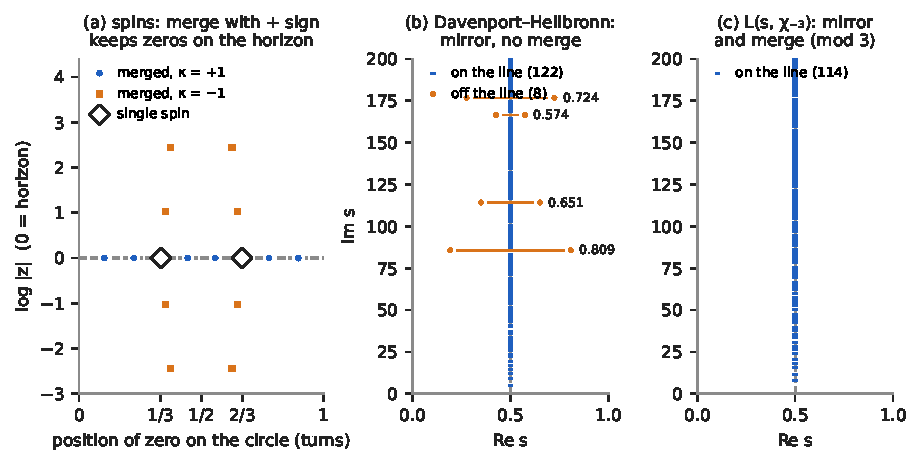
\includegraphics[width=\textwidth]{fig2_mirror.pdf}
\caption{(a) Lee--Yang zeros, plotted with $\log|z|=0$ as the horizon. A single three-state spin (diamonds) has zeros at exactly $\tfrac13$ and $\tfrac23$ of a turn. Four such spins merged with $\kappa=+1$ keep every zero on the horizon. Merged with $\kappa=-1$, the zeros leave it in mirrored pairs $z,1/\bar z$. (b) The Davenport--Heilbronn function has the mirror but not the merge: $122$ zeros on the line and four mirrored pairs off it below height $200$. (c) $L(s,\chi_{-3})$ has the mirror and the merge: $114$ zeros, all on the line.}\label{fig:mirror}
\end{figure}

\section{The merge inside \texorpdfstring{$\xi$}{xi}}\label{sec:xi}
We now build the merge into $\xi$ itself. The unit is a single random variable made of countably many independent pieces. Let $e_1,e_2,\dots$ be independent standard exponential variables and set
\[
S_1=\frac2{\pi^2}\sum_{n\ge1}\frac{e_n}{n^2},\qquad \mathbb E\,e^{-\beta S_1}=\frac{x}{\sinh x},\quad x=\sqrt{2\beta}.
\]
The Laplace transform follows from $\mathbb E\,e^{-\beta' e_n}=(1+\beta')^{-1}$ and Euler's product $\sinh x/x=\prod_{n\ge1}(1+x^2/\pi^2n^2)$. Merge two independent copies, $S_2=S_1\oplus S_1'$, so that $\mathbb E\,e^{-\beta S_2}=(x/\sinh x)^2$. A third law is the cosh unit $C_1=\frac2{\pi^2}\sum_{n\ge1}e_n/(n-\frac12)^2$, with $\mathbb E\,e^{-\beta C_1}=1/\cosh x$ by $\cosh x=\prod_{n\ge1}(1+x^2/\pi^2(n-\frac12)^2)$. For $\nu>0$, let $S_\nu=\frac2{\pi^2}\sum_{n\ge1}g_n/n^2$ with independent gamma variables $g_n$ of shape $\nu$ and scale $1$, so that $\mathbb E\,e^{-\beta' g_n}=(1+\beta')^{-\nu}$ and $\mathbb E\,e^{-\beta S_\nu}=(x/\sinh x)^\nu$. $S_\nu$ is the merge of $\nu$ copies; for integer $\nu$ it is the sum of $\nu$ independent copies of $S_1$, and $\nu$ need not be an integer. Write $M_\nu(s)=\mathbb E[(\pi S_\nu/2)^{s/2}]$. Since $S_\nu$ has exponential moments, $\mathbb E\,e^{\theta S_\nu}=(\sqrt{2\theta}/\sin\sqrt{2\theta})^\nu$ for $0\le\theta<\pi^2/2$, and its Laplace transform decays like $(2x)^\nu e^{-\nu x}$, $S_\nu$ has finite moments of every real order and $M_\nu$ is an entire function of $s$.

\begin{proposition}[Biane, Pitman and Yor]\label{prop:bpy}
The following identities hold \cite{BPY}.
\begin{enumerate}
\item $M_2(s)=\mathbb E\,[Y^s]=2\xi(s)$, where $Y=\sqrt{\pi S_2/2}$ is the merged pair.
\item $M_1(s)=2\xi(s)\,\dfrac{2^{1-s}-1}{1-s}$. A single copy carries $\xi$ times a factor built from the prime $2$ alone.
\item $\mathbb E[(\pi C_1/2)^{s/2}]=\Lambda_\beta(1+s)$, where $\Lambda_\beta(s)=(4/\pi)^{(s+1)/2}\Gamma(\tfrac{s+1}2)L(s,\chi_{-4})$ is the completed Dirichlet beta function of the four-cycle character.
\end{enumerate}
\end{proposition}
All three are reproduced numerically from the Laplace transforms. For $\alpha>0$, $\Gamma(\alpha)X^{-\alpha}=\int_0^\infty\beta^{\alpha-1}e^{-\beta X}\dd\beta$ gives
\[
\mathbb E[X^{-\alpha}]=\frac1{\Gamma(\alpha)}\int_0^\infty\beta^{\alpha-1}\,\mathbb E\,e^{-\beta X}\dd\beta ,
\]
and for $0<\alpha<1$, $X^\alpha=\frac \alpha{\Gamma(1-\alpha)}\int_0^\infty\beta^{-\alpha-1}(1-e^{-\beta X})\dd\beta$ gives the positive-moment branch
\[
\mathbb E[X^{\alpha}]=\frac \alpha{\Gamma(1-\alpha)}\int_0^\infty\beta^{-\alpha-1}\bigl(1-\mathbb E\,e^{-\beta X}\bigr)\dd\beta .
\]
We evaluated these by adaptive quadrature, and $\xi$ from $\zeta$ with $\xi(s)=\xi(1-s)$. At $s=-0.5,-1,-1.5,-2,-3,-4$ the ratios equal $1$ to ten digits. For example, $M_2(-1)=1.047197551197=2\xi(-1)=\pi/3$ (since $\xi(-1)=\xi(2)=\pi^{-1}\zeta(2)=\pi/6$), and $M_2(\tfrac14)=0.995678267772=2\xi(\tfrac14)$ on the positive-moment branch.

\begin{remark}[the single copy is the series of balanced pairs]\label{rem:eta}
Since $2\xi(s)=s(s-1)\pi^{-s/2}\Gamma(\frac s2)\zeta(s)$ and $s(s-1)(2^{1-s}-1)/(1-s)=s(1-2^{1-s})$, \cref{prop:bpy}(2) and \eqref{eq:eta} give
\[
M_1(s)=s\,\pi^{-s/2}\,\Gamma\bigl(\tfrac s2\bigr)\,\eta(s).
\]
The single unit is the completed alternating series of the pairs $(2k-1)^{-s}-(2k)^{-s}$ of \cref{sec:eta}. At $s=0$, $s\Gamma(\frac s2)\to2$ and $\eta(0)=\frac12$, the value of the elementary pair (\cref{prop:cycle}), so $M_1(0)=1$, as a moment of order zero must be. For example, $M_1(-1)=(-1)\pi^{1/2}\Gamma(-\frac12)\eta(-1)=\pi/2$, with $\Gamma(-\frac12)=-2\sqrt\pi$ and $\eta(-1)=-3\zeta(-1)=\frac14$, which is $\frac32M_2(-1)$.
\end{remark}

\begin{corollary}[two is exactly enough]\label{cor:two}
The single-copy function $M_1$ vanishes at $s=1+2\pi ik/\log2$ for $k\neq0$. These points lie on $\Re s=1$, and their images under $\iota$, on $\Re s=0$, are not zeros. Merging the pair removes this lattice exactly and leaves $\xi$, whose zeros are mirrored.
\end{corollary}
\begin{proof}
$2^{1-s}-1=0$ exactly when $(1-s)\log2\in2\pi i\mathbb Z$. The case $k=0$, $s=1$, cancels against $1-s$, and there $(2^{1-s}-1)/(1-s)\to\log2$. At a point $w=1-s=-2\pi ik/\log2$ the factor is $(2^{1-w}-1)/(1-w)=1/(1-w)\ne0$, and $\xi(w)=\xi(1+2\pi ik/\log2)\ne0$, because $\zeta$ has no zeros on $\Re s=1$ \cite[Ch.~III]{Titchmarsh} and the other factors of $\xi$ do not vanish there.
\end{proof}
Among merges of $\nu$ copies, the mirror $M_\nu=M_\nu\circ\iota$ holds only for the pair.
\begin{proposition}[only the pair has the mirror]\label{prop:onlytwo}
For every $\nu>0$, as $k\to\infty$ through the integers,
\[
\log\frac{M_\nu(1-2k)}{M_\nu(2k)}=2k\log\frac2\nu+o(k).
\]
Hence $M_\nu(s)=M_\nu(1-s)$ for all $s$ holds only at $\nu=2$, where it holds by \cref{prop:bpy}(1).
\end{proposition}
\begin{proof}
Write $X=S_\nu$ and $r=k-\frac12$. \emph{Positive moments.} All terms of $S_\nu$ are nonnegative, so $X\ge(2/\pi^2)g_1$ and $\mathbb E X^k\ge(2/\pi^2)^k\Gamma(k+\nu)/\Gamma(\nu)$. For $0<\theta<\pi^2/2$ and $x\ge0$, $x^k\le k!\,\theta^{-k}e^{\theta x}$, so $\mathbb E X^k\le k!\,\theta^{-k}\,\mathbb E\,e^{\theta X}$ with $\mathbb E\,e^{\theta X}<\infty$. Since $\theta$ may be taken as close to $\pi^2/2$ as we like, Stirling's formula gives $\log M_\nu(2k)=\log[(\pi/2)^k\,\mathbb E X^k]=k\log k-k-k\log\pi+o(k)$. \emph{Negative moments.} With $\beta=x^2/2$, $\mathbb E X^{-r}=2^{1-r}\Gamma(r)^{-1}\int_0^\infty x^{2r-1}(x/\sinh x)^\nu\dd x$. From $x/\sinh x=2xe^{-x}/(1-e^{-2x})$ we have $(2x)^\nu e^{-\nu x}\le(x/\sinh x)^\nu\le\min\{1,(1-e^{-2})^{-\nu}(2x)^\nu e^{-\nu x}\}$ for $x\ge1$, and $(x/\sinh x)^\nu\le1$ on $[0,1]$, so the integral equals $2^\nu\Gamma(2r+\nu)\nu^{-2r-\nu}e^{O(1)}$. Stirling's formula then gives $\log M_\nu(1-2k)=\log[(\pi/2)^{-r}\,\mathbb E X^{-r}]=k\log k-k-k\log\pi+2k\log(2/\nu)+O(\log k)$. Subtracting the two estimates proves the formula. For $\nu\ne2$ the right side tends to $\pm\infty$, so $M_\nu(1-2k)\ne M_\nu(2k)$ for large $k$.
\end{proof}
The ratio $M_\nu(s)/M_\nu(1-s)$ at $s=-0.6,-0.3,0.1,0.25$ is $2.239,1.797,1.341,1.201$ for $\nu=1$, and $0.99999999$--$1.00000000$ for $\nu=2$. It moves monotonically away from $1$ for $\nu=1.5,2.5,3,4$ (\cref{fig:merge}a). For $\nu=1$ these values also follow in closed form from \cref{prop:bpy}(2): $M_1(s)/M_1(1-s)=\frac{(2^{1-s}-1)/(1-s)}{(2^{s}-1)/s}$.

\paragraph{The first zero merges onto the line.} To evaluate $M_\nu$ at complex $s$ we use the positive-moment branch with $\alpha=s/2$, substitute $\beta=x^2/2$ and $x=e^v$, and split $1-(x/\sinh x)^\nu=(1-e^{-c_\nu x^2})+(e^{-c_\nu x^2}-(x/\sinh x)^\nu)$ with $c_\nu=\nu/6$, from $\log(x/\sinh x)=-x^2/6+x^4/180-\cdots$. The first part integrates in closed form, $\int_0^\infty x^{-2\alpha-1}(1-e^{-c_\nu x^2})\dd x=\frac12c_\nu^\alpha\,\Gamma(1-\alpha)/\alpha$, so that
\begin{equation}\label{eq:Mt}
M_\nu(s)=\Bigl(\frac\pi2\Bigr)^{\alpha}2^{\alpha+1}\biggl[\frac{c_\nu^\alpha}2+\frac{\alpha}{\Gamma(1-\alpha)}\int_{-\infty}^{\infty}e^{-2\alpha v}\Bigl(e^{-c_\nu e^{2v}}-\Bigl(\frac{e^v}{\sinh e^v}\Bigr)^\nu\Bigr)\dd v\biggr],\qquad \alpha=\frac s2 .
\end{equation}
The integrand is $O(e^{(4-2\Re\alpha)v})$ as $v\to-\infty$ and decays faster than exponentially as $v\to+\infty$, so \eqref{eq:Mt} holds for $\Re s<4$. We evaluate the integral by the trapezoidal rule on $-40\le v\le8$ with step $5\times10^{-4}$, computing the bracketed difference from the series of $\log(x/\sinh x)$ for $x<0.1$ to avoid cancellation. At $\nu=2$ this reproduces $2\xi$ to $7.5\times10^{-15}$ at $0.3+5i$. We then follow the zero through $\tfrac12+14.134725\,i$ as $\nu$ varies, in steps of $0.02$, solving $M_\nu(s)=0$ by a Newton-type iteration started from the zero found at the previous $\nu$; the residual $|M_\nu|$ on the path is at most $1.8\times10^{-12}$. An independent evaluation of $M_\nu$ by adaptive quadrature reproduces the path points below to $10^{-8}$.
\begin{itemize}
\item At $\nu=1$ the path ends at $1+9.064720\,i$, exactly the first prime-$2$ zero $1+2\pi i/\log2$.
\item Along the path, $\sigma$ decreases steadily: $0.914$ at $\nu=1.2$, $0.718$ at $1.6$, $0.611$ at $1.8$, $0.556$ at $1.9$.
\item It reaches the critical line at $\nu=2$, at $\tfrac12+14.134725\,i$, and crosses it there, to $0.443$ at $\nu=2.1$ and $-0.107$ at $\nu=3$.
\item On the whole path, $|\sigma-\tfrac12|<10^{-6}$ only at $\nu=2$.
\end{itemize}
The zero through $\gamma_2=21.022040$ is followed down to $\nu=1$ with residual below $4.4\times10^{-10}$, and it ends on $\xi$'s first zero, $\tfrac12+14.134725\,i$. As the two copies separate, the Riemann zeros step down by one, and the first leaves the line for the prime-$2$ lattice (\cref{fig:merge}b). We followed the zeros through $\gamma_1$ and $\gamma_2$ in double precision. For the first zero, the zero of the prime-$2$ pair on $\Re s=1$ is carried onto the horizon by the merge of the pair, and it sits there exactly when the merge is complete.

\paragraph{Riemann's kernel is the weighted logarithm of the merged pair.} From \cref{prop:bpy}(1), $\Xi(t)=\xi(\tfrac12+it)=\tfrac12\mathbb E[Y^{1/2}e^{it\log Y}]$. The law of $Y$ has the distribution function $\sum_{n\in\mathbb Z}(1-2\pi n^2y^2)e^{-\pi n^2y^2}$ \cite{BPY}. Differentiating term by term, $Y$ has density $f_Y(y)=2\sum_{n\ge1}(4\pi^2n^4y^3-6\pi n^2y)e^{-\pi n^2y^2}$, so $\log Y$ has density $f_{\log Y}(u)=e^uf_Y(e^u)=2\sum_{n\ge1}(4\pi^2n^4e^{4u}-6\pi n^2e^{2u})e^{-\pi n^2e^{2u}}$, and
\[
\Phi(u)=e^{u/2}f_{\log Y}(u).
\]
Consistently, $\frac12\int_\R\Phi(u)e^{izu}\dd u=\frac12\mathbb E[Y^{1/2+iz}]=\xi(\frac12+iz)=\Xi(z)$. By adaptive quadrature (for $y<\frac14$ we use $f_Y(y)=y^{-3/2}\Phi(\log y)$ and the evenness of $\Phi$), the density has total mass $1.000000000000$ and its moments reproduce $2\xi(s)$ at $s=-1,-0.5,0.25,0.5,2,3$ to within $1.3\times10^{-15}$. By Simpson's rule on $[-3,3]$ with step $10^{-4}$ ($\Phi(u)<10^{-190}$ for $|u|>2.5$), $\frac12\int_{-3}^3\Phi=0.497120778188=\xi(\tfrac12)$ and $\frac12\int_{-3}^3\Phi(u)\cos(\gamma_1u)\dd u=-4\times10^{-18}$. The Riemann spin of \cref{sec:horizon} is therefore the logarithm of the merged pair, weighted by $\sqrt Y$.

\begin{figure}[t]\centering
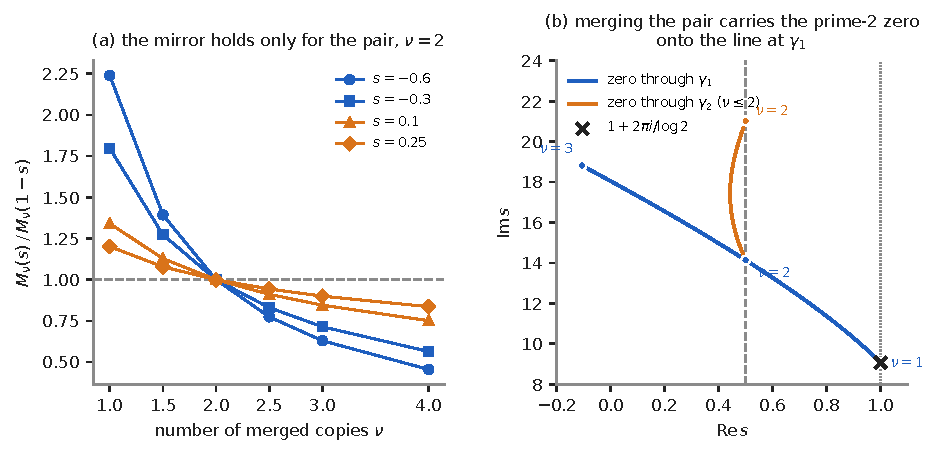
\includegraphics[width=\textwidth]{fig3_merge.pdf}
\caption{(a) The mirror ratio $M_\nu(s)/M_\nu(1-s)$ against the number of merged copies $\nu$. It equals $1$ only for the pair, $\nu=2$. (b) The zero through $\gamma_1$ followed in $\nu$. At $\nu=1$ it is the prime-$2$ zero $1+2\pi i/\log2$ (cross). It reaches the critical line (dashed) exactly at $\nu=2$, and crosses it. The zero through $\gamma_2$ descends to $\gamma_1$ as $\nu\to1$.}\label{fig:merge}
\end{figure}

\section{The signed current and the criterion}\label{sec:current}
The equivalence
\begin{equation}\label{eq:criterion}
\text{RH}\iff J(x,y)\ge0\quad\text{for all }x\in\R,\ y>0
\end{equation}
is the monotonicity criterion of Sondow and Dumitrescu \cite{SD}: $|\Xi(x+iy)|$ is nondecreasing in $y\ge0$ for every $x$. Since $J/H=4\Re\,\xi'/\xi(\frac12+y+ix)$ (\cref{prop:pairformula}), it is also the positivity criterion $\Re\,\xi'/\xi(s)>0$ on $\Re s>\frac12$ of Lagarias \cite{Lagarias}, who credits it to Hinkkanen. $H$ is even in $y$, the mirror $\mathsf R$ in the variable $z$, and $J$ is odd in $y$: the current measures how the pair balance of $\Xi$ changes as one moves off the fixed line of the mirror.

\paragraph{The kernel.} The series for $\Phi$ is even in $u$ (a consequence of the transformation formula of the theta function) and so represents $\Phi$ for all real $u$. For $u\ge0$ each term equals $4\pi n^2e^{5u/2}(2\pi n^2e^{2u}-3)e^{-\pi n^2e^{2u}}>0$, so $\Phi>0$, and $\Phi$ decays like $\exp(-\pi e^{2|u|})$; the series of absolute values, however, grows like $e^{|u|/2}$ as $u\to-\infty$. Adaptive quadrature of $\int_0^{3.2}\Phi(u)\cos(zu)\dd u$ in double precision, with the series truncated at $n\le12$, gives $\Xi(0)=0.4971207782$, equal to $\xi(\frac12)=-\frac18\pi^{-1/4}\Gamma(\frac14)\zeta(\frac12)$, and $|\Xi|<5\times10^{-18}$ at the first two zeros $\gamma_1,\gamma_2$ of \cref{sec:data}.

\begin{proposition}[pair formula]\label{prop:pairformula}
For $y>0$, $J/H=4\Re\,\xi'/\xi(\frac12+y+ix)=4\sum_w\frac{y-\Im w}{(x-\Re w)^2+(y-\Im w)^2}$, the sum over zeros $w$ of $\Xi$ taken in conjugate pairs. A pair $w=\gamma\mp ib$ ($b>0$) contributes
\[
\frac{8y\,(d^2+y^2-b^2)}{(d^2+(y-b)^2)(d^2+(y+b)^2)},\qquad d=x-\gamma,
\]
which is negative exactly on the open half-disk $d^2+y^2<b^2$; a real zero contributes $4y/(d^2+y^2)>0$. Consequently \eqref{eq:criterion} holds, and $\{J\le0\}\cap\{y>0\}$ is contained in the union of the closed half-disks of radius $b$ centred at $(\gamma,0)$ over nonreal zeros.
\end{proposition}
\begin{proof}
$\partial_y\log H=-2\Im(\Xi'/\Xi)$, so $J/H=-4\Im(\Xi'/\Xi)(x+iy)$. With $s=\frac12+i(x+iy)$, $\Xi'/\Xi=i\,\xi'/\xi(s)$, and the functional equation $\xi(s)=\xi(1-s)$ with $\xi(\bar s)=\overline{\xi(s)}$ gives $-\Re\xi'/\xi(\frac12-y+ix)=\Re\xi'/\xi(\frac12+y+ix)$. The Hadamard product of the even function $\Xi$ converges when zeros are taken with their negatives, which gives the sum; the pair term is elementary. If a zero $w=\gamma+ib$ with $b>0$ exists, $H(\gamma,b)=0$ while $J/H\to-\infty$ as $y\uparrow b$ at $x=\gamma$ (the pair term dominates), so $J<0$ somewhere; conversely with only real zeros every term is positive.
\end{proof}
The pair $\gamma\mp ib$ is a pair of mirror images under $\mathsf R$, and a real zero is fixed by $\mathsf R$: the current is negative only inside the half-disk spanned by a pair that the mirror has not merged into one zero.

\begin{proposition}[the unconditional region]\label{prop:region}
$J(x,y)>0$ if $|x|\le3\cdot10^{12}-\frac12$, or if $y\ge\frac12-1/(5.573412\,\log(|x|+\frac12))$.
\end{proposition}
\begin{proof}
All zeros with $|\gamma|\le3\cdot10^{12}$ are real \cite{PT}, so the half-disks of \cref{prop:pairformula} have centres $|\gamma|>3\cdot10^{12}$ and radii $<\frac12$. The zero-free region $\beta<1-1/(5.573412\log|\gamma|)$ \cite{MT} gives $b<\frac12-1/(5.573412\log|\gamma|)$; a point in a half-disk centred at $\gamma$ has $|\gamma|<|x|+\frac12$, so $y<b<\frac12-1/(5.573412\log(|x|+\frac12))$.
\end{proof}
So RH is equivalent to $J\ge0$ on
\[
\mathcal U=\Bigl\{|x|>3\cdot10^{12}-\tfrac12,\ \ 0<y<\tfrac12-\frac1{5.573412\log(|x|+\frac12)}\Bigr\};
\]
at $x=3\cdot10^{12}$ this leaves $98.75\%$ of the strip height open.

\section{The phase-space density}\label{sec:phase}
Define
\[
Q(p,x)=\int_\R\Phi\Bigl(\frac{p+q}2\Bigr)\Phi\Bigl(\frac{p-q}2\Bigr)\cos(xq)\,dq .
\]
With the Wigner function $W_\Phi(a,k)=\frac1{2\pi}\int_\R\Phi(a+\frac s2)\Phi(a-\frac s2)e^{-iks}ds$ of $\Phi$ regarded as an (unnormalised) wave function, $Q(p,x)=2\pi W_\Phi(p/2,x)$. $Q$ is real, even in $p$ and in $x$, and takes negative values, as it must by Hudson's theorem \cite{Hudson}, $\Phi$ not being Gaussian.

\begin{proposition}\label{prop:HJ}
$Q$ is real, even in $p$ and in $x$, $|Q(p,x)|\le Q(p,0)$, and for all $x\in\R$, $y\in\R$:
\[
H(x,y)=\frac18\int_\R Q(p,x)\cosh(yp)\,dp,\qquad J(x,y)=\frac14\int_\R Q(p,x)\,p\sinh(yp)\,dp .
\]
Moreover $\int_\R J(x,y)\,dx=4\pi\int_0^\infty\Phi(u)^2u\sinh(2yu)\dd u>0$ for every $y>0$, whatever the zeros.
\end{proposition}
\begin{proof}
$H=\frac14\iint\Phi(u)\Phi(v)e^{izu-i\bar zv}du\,dv$ with $z=x+iy$. Substitute $p=u+v$, $q=u-v$ ($du\,dv=\frac12dp\,dq$); then $izu-i\bar zv=ixq-yp$, and the parts odd in $q$ vanish by the symmetry $q\to-q$ of $\Phi(\frac{p+q}2)\Phi(\frac{p-q}2)$. This gives $H=\frac18\int Q\,e^{-yp}dp$, and evenness of $Q$ in $p$ turns $e^{-yp}$ into $\cosh(yp)$; differentiate for $J$. $|Q(p,x)|\le Q(p,0)$ because $\Phi>0$. The last statement is Plancherel in $x$: $\int|\Xi(x+iy)|^2dx=\pi\int_0^\infty\Phi^2\cosh(2yu)\dd u$, differentiated in $y$.
\end{proof}
Pooling the current over $x$ can never detect a zero off the line: the sign question is local in $x$. RH is thus a statement about how the negative part of a Wigner function is weighted. Substituting $p=2a$ in \cref{prop:HJ}, $J(x,y)=2\pi\int_\R W_\Phi(a,x)\,a\sinh(2ya)\,da=2\pi\langle\Phi|\hat O_{x,y}|\Phi\rangle$, where $\hat O_{x,y}$ is the observable with Weyl symbol $a\sinh(2ya)\,\delta(k-x)\ge0$. With the normalised state $\varphi=\Phi/\|\Phi\|$ this reads $J=2\pi\|\Phi\|^2\langle\varphi|\hat O_{x,y}|\varphi\rangle$, the form in which the companion paper \cite{SQuant} studies $J$ as a quantum expectation.

\section{The exact expansion}\label{sec:expansion}

\begin{theorem}[Macdonald expansion]\label{thm:macdonald}
For all real $p,x$, with $z_N=2\pi Ne^p$,
\[
Q(p,x)=8e^{p/2}\sum_{N\ge1}\tau_x(N)\,\mathcal K_x(z_N),\qquad \mathcal K_x(z)=(z^4+9z^2)K_{ix}(z)+6z^3K'_{ix}(z),
\]
\[
\tau_x(N)=\sum_{mn=N}\cos\Bigl(x\log\frac mn\Bigr)=N^{-ix}\sigma_{2ix}(N)=\sum_{d\mid N}\Bigl(\frac{d^2}{N}\Bigr)^{ix},
\]
where $K_{ix}(z)=\int_0^\infty e^{-z\cosh w}\cos(xw)dw$ is the Macdonald function of imaginary order, real for $z>0$, and $\sum_N\tau_x(N)N^{-s}=\zeta(s+ix)\zeta(s-ix)$ for $\Re s>1$.
\end{theorem}
\begin{proof}
Insert the series for $\Phi(u)$ and $\Phi(v)$, valid for all real arguments by evenness. The resulting double series in $(m,n)$ may be integrated termwise: with $u=\frac{p+q}2$, $v=\frac{p-q}2$, the series of absolute values is $O(e^{|u|/2})$ in $u$ and $O(e^{|v|/2})$ in $v$ and doubly-exponentially small in whichever of $u,v$ is positive, so for fixed $p$ the absolute double series is dominated by an integrable function of $q$. The exponent is $-\pi(m^2e^{2u}+n^2e^{2v})=-\pi e^p(m^2e^q+n^2e^{-q})=-z\cosh(q+c)$, $z=2\pi mne^p$, $c=\log\frac mn$. The four prefactors are $16$ times $4\pi^4m^4n^4e^{9p/2}$, $-6\pi^3m^4n^2e^{7p/2}e^{q}$, $-6\pi^3m^2n^4e^{7p/2}e^{-q}$, $9\pi^2m^2n^2e^{5p/2}$. Put $w=q+c$ and use $\int_\R e^{-z\cosh w}e^{\omega w}dw=2K_\omega(z)$, valid for complex order $\omega$ \cite[10.32.9]{DLMF}. The terms in $e^{\pm q}$ give $e^{\mp c}\cdot2\Re[e^{-ixc}K_{1\pm ix}(z)]$; the factors $e^{\mp c}=(n/m)^{\pm1}$ turn both coefficients into $(mn)^3$, and $K_{1-ix}=\overline{K_{1+ix}}$ on $z>0$, so the two combine to $4\cos(xc)\Re K_{1+ix}(z)$, the $\sin(xc)$ parts cancelling pair by pair. Finally $\Re K_{1+ix}(z)=\int_0^\infty e^{-z\cosh w}\cosh w\cos(xw)dw=-K'_{ix}(z)$. Collecting with $m^2n^2e^{2p}=z^2/4\pi^2$ gives the display; summing over $mn=N$ gives $\tau_x(N)$. The three expressions for $\tau_x$ agree because $d\leftrightarrow N/d$ pairs conjugate summands.
\end{proof}

\begin{proposition}[operator form]\label{prop:operator}
With $D=z\,d/dz$, $\mathcal K_x=((D+1)^2+x^2)(D^2+x^2)K_{ix}$. With $E^*(z,s)=\pi^{-s}\Gamma(s)\zeta(2s)E(z,s)$ the completed Eisenstein series for $\mathrm{SL}_2(\mathbb Z)$,
\[
Q(p,x)=2\Bigl(\bigl(\partial_p+\tfrac12\bigr)^2+x^2\Bigr)\Bigl(\bigl(\partial_p-\tfrac12\bigr)^2+x^2\Bigr)E^*\bigl(ie^p,\tfrac12+ix\bigr).
\]
\end{proposition}
\begin{proof}
Bessel's equation reads $D^2K_{ix}=(z^2-x^2)K_{ix}$, i.e.\ $z^2K_{ix}=(D^2+x^2)K_{ix}$, and $z^2D=(D-2)z^2$. Hence $z^4K_{ix}=((D-2)^2+x^2)(D^2+x^2)K_{ix}$ and $z^3K'_{ix}=z^2DK_{ix}=(D-2)(D^2+x^2)K_{ix}$, and $(D-2)^2+x^2+9+6(D-2)=(D+1)^2+x^2$. For the second statement, the Fourier expansion \cite[\S3.4]{Iwaniec} gives, at $s=\frac12+ix$ and $z=iy$,
\[
E^*(iy,s)=\zeta^*(2s)y^s+\zeta^*(2-2s)y^{1-s}+4\sqrt y\sum_{N\ge1}\tau_x(N)K_{ix}(2\pi Ny),\qquad\zeta^*(w)=\pi^{-w/2}\Gamma(\tfrac w2)\zeta(w).
\]
On functions of $p=\log y$, $D$ acts as $\partial_p$ on each term of \cref{thm:macdonald}, and $e^{p/2}\partial_p=(\partial_p-\frac12)e^{p/2}$, so $Q=8((\partial_p+\frac12)^2+x^2)((\partial_p-\frac12)^2+x^2)\bigl[e^{p/2}\sum_N\tau_x(N)K_{ix}(2\pi Ne^p)\bigr]$. The constant terms $y^{\frac12\pm ix}=e^{(\frac12\pm ix)p}$ are annihilated by $(\partial_p-\frac12)^2+x^2$.
\end{proof}
The evenness of $Q$ in $p$ is the invariance $E^*(i/y,s)=E^*(iy,s)$ together with the invariance of the operator under $\partial_p\mapsto-\partial_p$: the mirror of the functional equation, seen in phase space, is the modular inversion $y\mapsto1/y$. In double precision, the expansion above, with $\zeta^*(1+2ix)$ from Euler--Maclaurin summation (\cref{sec:methods}) and $K_{ix}$ by the trapezoidal rule, satisfies $E^*(i/y)=E^*(iy)$ to relative $5\times10^{-14}$ at $(x,y)=(3,0.8),(5,0.6),(9,0.9)$, which fixes its normalisation; and with $D$ (respectively $\partial_p$) replaced by 9-point central differences of step $0.02$ in $\log z$ (respectively $p$), the two operator identities hold to $7\times10^{-8}$ at $(x,z)=(3,2),(3,6),(7,4),(7,12)$ and to $9\times10^{-9}$ at $(p,x)=(0.3,3),(-0.2,5)$, the accuracy of fourth derivatives taken by finite differences of this step.

\paragraph{Numerical evaluation of the expansion.} The expansion (terms with $z_N\le700$; $K_{ix}$ and $K'_{ix}$ by adaptive quadrature of their integral representations) agrees with direct adaptive quadrature of the defining integral of $Q$ over $|q|\le6.5$, both in double precision, at the seven points $(p,x)=(0,0)$, $(0,3)$, $(0.2,13)$, $(-0.7,5)$, $(0.9,7)$, $(1.5,2)$, $(0.4,10)$: the relative differences are $1.9\times10^{-16}$ to $2.4\times10^{-14}$ at six of them, and $1.9\times10^{-12}$ at the seventh, the Wigner-negative point $Q(0.2,13)=-2.0918537524\times10^{-4}$. At $x=50$, where $|Q|<10^{-26}$ and double-precision quadrature fails, we computed $J=\frac12\int_0^4Q\,p\sinh(yp)\,dp$ by the trapezoidal rule of step $0.01$ with $Q$ from the expansion in 80-digit arithmetic, and independently $J=-4\Im(\bar\Xi\,\Xi')$ with $\Xi,\Xi'$ from the kernel integral (\cref{sec:methods}); the two agree to relative $1.3$--$1.8\times10^{-15}$ at $y=0.1,0.5,1$.

\paragraph{Two regimes.} Put $a=\sqrt{x^2+\frac14}$ and $\mathcal B(z)=\sqrt zK_{ix}(z)$, so that $\mathcal B''=(1-a^2/z^2)\mathcal B$. For $z<a$, $\mathcal B$ oscillates; for $z\ge a$ it is positive and decreasing (\cref{lem:riccati}). For $z<x$ the leading steepest-descent term is
\begin{equation}\label{eq:debye}
K_{ix}(z)\approx\sqrt{2\pi}\,(x^2-z^2)^{-1/4}e^{-\pi x/2}\cos\Bigl(x\,\mathrm{arccosh}\frac xz-\sqrt{x^2-z^2}-\frac\pi4\Bigr),
\end{equation}
with uniform expansions and error bounds due to Dunster \cite{Dunster}; at $x=50$ the ratio of $K_{ix}$ (computed in 80-digit arithmetic, \cref{sec:methods}) to \eqref{eq:debye} is $1.0006,0.990,0.996,1.0008,0.378,1.012,1.027,0.896$ at $z=2,5,10,20,30,40,45,48$ (at $z=30$, $K_{ix}$ is near a zero; at $z=48$ the leading term fails near the turning point). At Wigner position $p$ the expansion is therefore a trigonometric sum of amplitude $e^{-\pi x/2}$ over the divisor-weighted $N<x/(2\pi e^p)$, followed by an Airy transition at $N\approx x/(2\pi e^p)$ and a doubly-exponentially small tail. At $p=0$ the oscillatory range is the hyperbola $mn<x/2\pi$ of the approximate functional equation for $|\zeta(\frac12+ix)|^2$.

\section{Mellin duality and the moments}\label{sec:mellin}

\begin{theorem}[Mellin duality]\label{thm:mellin}
For all $w\in\C$,
\[
\mathcal F(w):=\int_\R Q(p,x)\,e^{(w-\frac12)p}\,dp=8\,\xi(w+ix)\,\xi(w-ix).
\]
For $\Re w>0$ the Mellin transform of $\mathcal K_x$ is $\int_0^\infty t^{w-1}\mathcal K_x(t)\,dt=2^{w-2}\,s_+(s_+-1)\,s_-(s_--1)\,\Gamma(\frac{s_+}2)\Gamma(\frac{s_-}2)$ with $s_\pm=w\pm ix$, and $9$, $6$ are the only weights for which the multiplier is this completing factor.
\end{theorem}
\begin{proof}
$\mathcal F$ is entire because $Q$ decays doubly exponentially in $|p|$. By \cite[10.43.19]{DLMF}, $\mathcal M_K(w):=\int_0^\infty t^{w-1}K_{ix}(t)dt=2^{w-2}\Gamma(\frac{s_+}2)\Gamma(\frac{s_-}2)$ for $\Re w>0$, and integration by parts gives $\mathcal M[Df](w)=-w\mathcal M[f](w)$ for $f=D^jK_{ix}$, $j\le3$ (the boundary terms $[t^wf(t)]_0^\infty$ vanish for $\Re w>0$, because each $D^jK_{ix}(t)$ is $O(1+|\log t|)$ as $t\to0$ and decays like $e^{-t}$ as $t\to\infty$). By \cref{prop:operator},
\[
\mathcal M[\mathcal K_x](w)=\bigl((1-w)^2+x^2\bigr)\bigl(w^2+x^2\bigr)\mathcal M_K(w)=(s_+-1)(s_--1)\,s_+s_-\,\mathcal M_K(w).
\]
With weights $c_1,c_2$ in place of $9,6$ the first factor is $D^2+(c_2-4)D+4+x^2+c_1-2c_2$, which equals $(D+1)^2+x^2$ only for $(c_1,c_2)=(9,6)$. On $\Re w>1$ insert \cref{thm:macdonald} term by term (absolute convergence of $\sum\tau_x(N)N^{-w}$ and of each Bessel integral); with $(2\pi)^{-w}2^{w-2}=\frac14\pi^{-w}$ this gives $8\cdot\frac12s_+(s_+-1)\pi^{-s_+/2}\Gamma(\frac{s_+}2)\zeta(s_+)\cdot\frac12s_-(s_--1)\pi^{-s_-/2}\Gamma(\frac{s_-}2)\zeta(s_-)$. Both sides are entire and agree on $\Re w>1$.
\end{proof}
This is Hecke's integral representation, applied to the Eisenstein series of \cref{prop:operator} (cf.\ \cite[Ch.~3]{Iwaniec}). For real $w$ the closed form reads $\mathcal M_K(w+4)+9\mathcal M_K(w+2)-6(w+2)\mathcal M_K(w+2)=2^{w-2}|s(s-1)|^2|\Gamma(\frac s2)|^2$, $s=w+ix$, where the left side uses $\mathcal M[z^4K_{ix}](w)=\mathcal M_K(w+4)$, $\mathcal M[z^2K_{ix}](w)=\mathcal M_K(w+2)$ and $\mathcal M[z^3K'_{ix}](w)=-(w+2)\mathcal M_K(w+2)$. In double precision, with $\mathcal M_K$ from \cite[10.43.19]{DLMF}, the two sides agree to relative $10^{-13}$ at $(w,x)=(1.5,0)$ and $1$--$7\times10^{-15}$ at $(1.5,3)$, $(2,10)$, $(3.2,\gamma_1)$, $(1.1,25)$; adaptive quadrature of $\int_{10^{-6}}^{60}t^{w-1}\mathcal K_x(t)\,dt$ agrees with the closed form to $4\times10^{-15}$ at $(w,x)=(1.5,3)$ and $(2,5)$.

For real $w=\frac12+y$, $\xi(\frac12+y+ix)\xi(\frac12+y-ix)=|\xi(\frac12-y+ix)|^2=H(x,y)$, so \cref{thm:mellin} contains \cref{prop:HJ}. Differentiating $\mathcal F$ at $w=\frac12$:

\begin{theorem}[moments]\label{thm:moments}
For $k\ge0$, $\int_\R Q(p,x)p^{2k}dp=8\,\partial_y^{2k}H(x,y)\big|_{y=0}=8(2k)!\,h_k(x)$, where $h_k(x)$ is the coefficient of $y^{2k}$ in $H(x,y)=|\Xi(x+iy)|^2$; in particular $h_0=\Xi^2$ and $h_1=\Xi'^2-\Xi\Xi''$, and
\[
\lim_{y\to0}\frac{J(x,y)}{y}=4\bigl(\Xi'(x)^2-\Xi(x)\Xi''(x)\bigr)=\frac14\int_\R Q(p,x)\,p^2\,dp .
\]
The following are equivalent: (a) RH; (b) $\int_\R Q(p,x)p^{2k}dp\ge0$ for all $k\ge0$ and all $x\in\R$.
\end{theorem}
\begin{proof}
The identities are Taylor's theorem applied to $\mathcal F(\frac12+y)=8H(x,y)$, an entire function of $y$. (a)$\Rightarrow$(b): if all zeros $\pm\gamma$ of $\Xi$ are real, $\Xi(z)=\Xi(0)\prod_{\gamma>0}(1-z^2/\gamma^2)$ (absolutely convergent), and for real $x$
\[
H(x,y)=\Xi(0)^2\prod_{\gamma>0}\frac{\bigl((\gamma-x)^2+y^2\bigr)\bigl((\gamma+x)^2+y^2\bigr)}{\gamma^4}.
\]
Each factor is a polynomial in $y^2$ with nonnegative coefficients, the product converges locally uniformly in $y$, and so every Taylor coefficient $h_k(x)$ of the limit is nonnegative. (b)$\Rightarrow$(a): if every $h_k(x)\ge0$, then $H(x,y)=\sum_kh_k(x)y^{2k}$ is nondecreasing in $y\ge0$, so $J\ge0$ for $y>0$, and RH follows from \cref{prop:pairformula}.
\end{proof}
The same equivalence, in the language of generalised Laguerre inequalities, is due to Patrick \cite{Patrick} and Csordas--Varga \cite[Thm.~2.9]{CV}. In 80-digit arithmetic, at $x=0,3,10,\gamma_1,17$, the value $4(\Xi'^2-\Xi\Xi'')$ with $\Xi,\Xi',\Xi''$ from the kernel integral and the value $\frac14\int_\R Q\,p^2dp=\frac12\int_0^{4.5}Q\,p^2dp$ by the trapezoidal rule of step $0.005$ with $Q$ from \cref{thm:macdonald} agree to 16 significant digits. Since $J/y=4h_1+8h_2y^2+O(y^4)$, the ratio $(J/y-4h_1)/4h_1$, with $J$ from the kernel integral, scales like $y^2$: it is $4.5\times10^{-8}$ to $1.6\times10^{-7}$ at $y=10^{-3}$ and $100$ times smaller, to four significant digits, at $y=10^{-4}$. In Wigner language: RH holds iff, at every fixed momentum, every even position moment of the kernel's Wigner function is nonnegative. The case $k=1$ is Laguerre's inequality $\Xi'^2-\Xi\Xi''\ge0$, a necessary condition for RH.

\section{The Euler product of the Wigner coefficients}\label{sec:euler}

For a prime $\ell$ let $\theta_\ell=2\pi\|x\log\ell/2\pi\|$ and $\phi_\ell=2\pi\|x\log\ell/2\pi-\frac12\|$, the distances in $[0,\pi]$ of the phase $x\log\ell$ from $0$ and from $\pi$ modulo $2\pi$. Thus $\theta_\ell=0$ exactly when $1-\ell^{-ix}=0$, that is, when $ix$ lies on the lattice of the Euler factor at $\ell$ (\cref{sec:eta}), and $\phi_\ell=0$ exactly when $1+\ell^{-ix}=0$, a pole of the local factor $(1+\ell^{-s})^{-1}$ of $\sum\lambda(n)n^{-s}$ (\cref{sec:balance}).

\begin{theorem}\label{thm:euler}
$\tau_x$ is multiplicative, and for every prime $\ell$ and $k\ge0$,
\begin{gather*}
\tau_x(\ell^k)=U_k\bigl(\cos(x\log\ell)\bigr)=\frac{\sin((k+1)x\log\ell)}{\sin(x\log\ell)},\\
\sum_{N\ge1}\frac{\tau_x(N)}{N^s}=\prod_\ell\frac1{1-2\cos(x\log\ell)\,\ell^{-s}+\ell^{-2s}}\qquad(\Re s>1),
\end{gather*}
where $U_k$ is the Chebyshev polynomial of the second kind; for real $s=\sigma>1$ each local factor equals $|1-\ell^{-\sigma-ix}|^{-2}>0$. For $N=\prod_\ell\ell^{k_\ell}$:
\begin{enumerate}
\item (aligned phases) if $k_\ell(k_\ell+2)\theta_\ell^2\le6$ for every $\ell\mid N$, then
\[
\frac{\tau_x(N)}{d(N)}\ \ge\ \prod_{\ell\mid N}\Bigl(1-\frac{k_\ell(k_\ell+2)\,\theta_\ell^2}6\Bigr)\ \ge\ 0;
\]
\item (alternating phases) if $k_\ell(k_\ell+2)\phi_\ell^2\le6$ for every $\ell\mid N$, then
\[
\frac{\tau_x(N)}{\lambda(N)d(N)}\ \ge\ \prod_{\ell\mid N}\Bigl(1-\frac{k_\ell(k_\ell+2)\,\phi_\ell^2}6\Bigr)\ \ge\ 0.
\]
\end{enumerate}
\end{theorem}
\begin{proof}
$\tau_x(N)=N^{-ix}\sigma_{2ix}(N)$ is a product of multiplicative functions. For $N=\ell^k$, $\tau_x(\ell^k)=\sum_{j=0}^ke^{i(2j-k)\varphi}$ with $\varphi=x\log\ell$, which is $\sin((k+1)\varphi)/\sin\varphi=U_k(\cos\varphi)$. The generating function $\sum_kU_k(c)T^k=(1-2cT+T^2)^{-1}$ with $T=\ell^{-s}$ gives the product, and $1-2\cos\varphi\,T+T^2=|1-Te^{i\varphi}|^2$ for real $T$. For the bounds, $U_k(\cos\varphi)$ depends only on $\cos\varphi=\cos\theta_\ell$, and with $n=k+1$,
\[
\frac{\sin n\theta}{n\sin\theta}=\frac1n\sum_{j=0}^{n-1}\cos\bigl((n-1-2j)\theta\bigr)\ge1-\frac{\theta^2}{2n}\sum_{j=0}^{n-1}(n-1-2j)^2=1-\frac{(n^2-1)\theta^2}6 ;
\]
multiply over $\ell\mid N$, all factors being nonnegative. For (2), $\cos(x\log\ell)=-\cos\phi_\ell$ and $U_k(-c)=(-1)^kU_k(c)$.
\end{proof}
For $x\ne0$ at most one prime can have $\theta_\ell=0$ exactly, since no two of the lattices of \cref{sec:eta} share a point other than $0$, so the bounds are the useful form; by Dirichlet's and Kronecker's theorems there are heights at which all $\theta_\ell$, respectively all $\phi_\ell$, for $\ell\le L$ are simultaneously below any $\varepsilon>0$.

\paragraph{The bounds at aligned and alternating heights.} At the six heights of \cref{sec:heights}, rounded to $10^{-3}$ as quoted there, direct enumeration of divisors in double precision shows that the side conditions $k_\ell(k_\ell+2)\theta_\ell^2\le6$ (respectively $k_\ell(k_\ell+2)\phi_\ell^2\le6$) hold for all 242 13-smooth $N\le1000$, and the bounds hold for each of them; the smallest bounds are $\tau_x(N)/d(N)\ge0.927,0.736,0.575$ at the three aligned heights (observed minima $0.929,0.756,0.626$) and $\tau_x(N)/(\lambda(N)d(N))\ge0.498,0.865,0.864$ at the three alternating ones (observed $0.568,0.870,0.869$). At $x=123456.789$ direct summation over divisors gives $\tau_x(2^5)=-5.5312244925$, $\tau_x(3^4)=-1.1567144745$, $\tau_x(7^3)=0.7341540313$, each equal to $U_k(\cos(x\log\ell))$ to $10^{-10}$, the limit set by double-precision phases $x\log d$ at this height.

\begin{remark}[the two camps]\label{rem:camps}
$\lambda$ is the unique completely multiplicative function equal to $-1$ on every prime: on the divisibility graph, in which $n$ and $n\ell$ are joined, it is the $\pm1$ labelling that changes sign across every edge. Its two classes (even and odd $\Omega$) are balanced in the sense $L(x)=O(x^{1/2+\varepsilon})$ for every $\varepsilon>0$ iff RH holds (\cref{prop:RH}; \cite[Thm.~1.2]{Borwein}). \Cref{thm:euler} says that the Wigner coefficients interpolate, height by height, between the unsigned divisor function (phases aligned) and this balanced signing (phases alternating). \Cref{sec:heights} measures the margin of \eqref{eq:criterion} near both extremes.
\end{remark}

\section{Where the density is positive}\label{sec:positive}

With $a=\sqrt{x^2+\frac14}$ and $\mathcal B(z)=\sqrt z\,K_{ix}(z)$ we have $\mathcal B''=c(z)\mathcal B$ with $c=1-a^2/z^2$, increasing in $z$.

\begin{lemma}[Riccati bounds]\label{lem:riccati}
For $z\ge a$: $K_{ix}(z)>0$, $K'_{ix}(z)<0$, and with $r=-\mathcal B'/\mathcal B$,
\begin{gather*}
\sqrt{c(z)}\le r(z)\le1,\qquad 0<-\frac{K'_{ix}(z)}{K_{ix}(z)}\le1+\frac1{2z},\\
K_{ix}(z)\ge\sqrt{\frac\pi{2z}}\exp\Bigl(-\sqrt{z^2-a^2}-a\arcsin\frac az\Bigr).
\end{gather*}
\end{lemma}
\begin{proof}
On $[a,\infty)$, $c\ge0$, so $\mathcal B$ has at most one zero there (between two zeros $\mathcal B$ would be positive and convex, or negative and concave). As $z\to\infty$, $K_{ix}(z)=\sqrt{\pi/2z}\,e^{-z}(1+O(1/z))$ \cite[10.40.2]{DLMF}, so $\mathcal B\to0^+$. If $\mathcal B(z_0)=0$ for some $z_0\ge a$, then on $(z_0,\infty)$ $\mathcal B$ has one sign, say positive, with $\mathcal B''\ge0$ and $\mathcal B'(z_0)>0$ by uniqueness, so $\mathcal B$ increases, contradicting $\mathcal B\to0$. Hence $\mathcal B>0$, and convexity with $\mathcal B\to0$ gives $\mathcal B'<0$. Then $r>0$ is finite and $r'=r^2-c$. If $r(z_0)>1$, comparison with the solution of $v'=v^2-1$ forces blow-up at finite $z$; if $r(z_0)<\sqrt{c(z_0)}$, then $r<\sqrt c$ persists (since $r$ decreases while $\sqrt c$ increases) and $r'\le r(z_0)^2-c(z_0)<0$ drives $r$ negative. Both contradict $0<r<\infty$. The ratio bound is $-K'/K=r+1/(2z)$. For the lower bound integrate $(\log\mathcal B)'\le-\sqrt c$ from $z$ to $Z$, use $\int_z^Z\sqrt c=[\sqrt{s^2-a^2}-a\arccos(a/s)]_z^Z$ and $\mathcal B(Z)=\sqrt{\pi/2}\,e^{-Z}(1+o(1))$, and let $Z\to\infty$.
\end{proof}

\begin{theorem}[tail positivity]\label{thm:tail}
Let $z_1=2\pi e^p$ and $z_0=\max(\sqrt2\,a,20)$. If $z_1\ge z_0$ then
\[
Q(p,x)\ge8(1-10^{-4})\,e^{p/2}z_1^2(z_1^2-6z_1+6)K_{ix}(z_1)>0 .
\]
Hence every negative value of $Q(\cdot,x)$ lies at $|p|<p_0(x):=\log(z_0/2\pi)$, which is $\log(x/2\pi)+\frac12\log2+O(x^{-2})$ for $|x|\ge14.14$.
\end{theorem}
\begin{proof}
By \cref{lem:riccati}, for $z\ge a$, $\mathcal K_x(z)\ge K_{ix}(z)[z^4+9z^2-6z^3(1+\frac1{2z})]=K_{ix}(z)z^2(z^2-6z+6)$, positive for $z>3+\sqrt3$, and $|\mathcal K_x(z)|\le K_{ix}(z)(z^4+6z^3+12z^2)$. Also $|\tau_x(N)|\le d(N)$, $\tau_x(1)=1$, and $(\log\mathcal B)'\le-\sqrt c\le-1/\sqrt2$ on $[z_1,\infty)$ when $z_1\ge\sqrt2a$, so $K_{ix}(Nz_1)\le K_{ix}(z_1)N^{-1/2}e^{-(N-1)z_1/\sqrt2}$. Keeping the $N=1$ term exactly, bounding each term $N\ge2$ in absolute value by $d(N)K_{ix}(Nz_1)(N^4z_1^4+6N^3z_1^3+12N^2z_1^2)$, and dropping the factor $N^{-1/2}\le1$, we get $Q\ge8e^{p/2}K_{ix}(z_1)z_1^2(z_1^2-6z_1+6)(1-R(z_1))$ with
\[
R(z)=\frac{\sum_{N\ge2}d(N)(N^4z^4+6N^3z^3+12N^2z^2)e^{-(N-1)z/\sqrt2}}{z^2(z^2-6z+6)} .
\]
The logarithmic derivative of each numerator term is at most $4/z$ (the polynomial has degree $4$ with positive coefficients, and the exponential factor decreases), while that of the denominator is $2/z+(2z-6)/(z^2-6z+6)\ge4/z$ for $z>3+\sqrt3=4.73$. So every term of $R$ decreases on $[20,\infty)$, and $R(z_1)\le R(20)=3.74\times10^{-5}$ (the crude bound $d(N)\le N$ gives $R(20)<4.4\times10^{-5}$).
\end{proof}

\begin{figure}[t]\centering
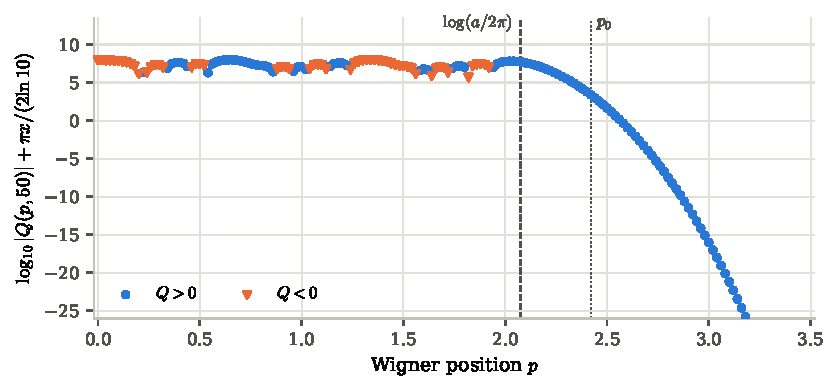
\includegraphics[width=0.92\textwidth]{fig4_sign_structure.pdf}
\caption{Sign and size of $Q(p,50)$, scaled by $e^{\pi x/2}$, on a grid of step $0.02$ in 95-digit arithmetic. Negative values (triangles) occur only for $p<1.93$, before the $N=1$ turning point $\log(a/2\pi)=2.074$ (dashed) and the proved threshold $p_0=2.421$ (dotted) of \cref{thm:tail}.}
\label{fig:sign}
\end{figure}

\paragraph{The sign of $Q$ at $x=50$, $100$ and $200$.} At $x=50$ and $z/a=1.0005,1.01,1.05,1.2,1.5,2,3,5$, with $K_{ix}$ and $K'_{ix}$ in 90-digit arithmetic, the bounds of \cref{lem:riccati} hold and the ratio of $K_{ix}$ to its lower bound decreases from $2.15$ to $1.01$. We scanned the sign of $Q(\cdot,x)$ (\cref{fig:sign}), evaluated from \cref{thm:macdonald} in $60+0.7x$ significant digits (95, 130 and 200 digits; see \cref{sec:methods} for why the precision must grow with $x$), on $p\in[0,3.5]$ with step $0.02$ at $x=50$ and on $p\in[-1.5,\log(x/2\pi)+1.6]$ with step $0.05$ at $x=100,200$ (by evenness this covers $|p|$ in the same ranges). The last negative grid value is at $p=1.92$ ($x=50$), $2.65$ ($x=100$) and $3.40$ ($x=200$), against $p_0=2.42,3.11,3.81$: negativity ends where the $N=1$ term leaves its oscillatory regime. Evaluating $R$ on a grid of step $0.1$ over $[20,200]$ (with the sum over $N\le399$, the omitted terms being below $e^{-5000}$) shows it decreasing, as proved above, with $R(20)=3.7369\times10^{-5}$.

\begin{corollary}[the reach of kernel-only positivity]\label{cor:calib}
$J(x,y)>0$ whenever $|x|\ge14.15$ and $y\ge5.24\sqrt{x^2+\frac14}$, and whenever $|x|<14.15$ and $y\ge64$.
\end{corollary}
\begin{proof}
By evenness, $J=\frac12\int_0^\infty Q\,p\sinh(yp)dp$; split at $p_0=\log(z_0/2\pi)$, $z_0=\max(\sqrt2a,20)$.

\emph{Head.} On $0\le p<p_0$, $|Q(p,x)|\le Q(p,0)$ and $0\le p\sinh(yp)\le\frac12p_0e^{yp_0}$, while $\int_0^\infty Q(p,0)dp=4H(0,0)=4\Xi(0)^2=0.98852<0.9886$ by \cref{prop:HJ} and $\Xi(0)=0.4971208$. So the head is at least $-\frac12\cdot\frac12p_0e^{yp_0}\cdot0.9886\ge-0.2472\,p_0e^{yp_0}=-0.2472\,p_0(z_0/2\pi)^y$.

\emph{Tail.} On $p\ge p_0$ we have $z_1=2\pi e^p\ge z_0\ge20$, so \cref{thm:tail} applies, and $z_1^2-6z_1+6\ge z_1^2(1-\frac6{20})\ge0.7z_1^2$. Since $\sqrt{z^2-a^2}\le z$ and $\arcsin(a/z)\le\pi/2$, \cref{lem:riccati} gives $K_{ix}(z_1)\ge\sqrt{\pi/2z_1}\,e^{-z_1-\pi a/2}$. If $yp_0\ge2$ then $p\sinh(yp)=\frac12pe^{yp}(1-e^{-2yp})\ge\frac12(1-e^{-4})p_0e^{yp}\ge0.49\,p_0e^{yp}$. Substituting $s=2\pi e^p$ ($dp=ds/s$, $e^{p/2}=(s/2\pi)^{1/2}$, $e^{yp}=(s/2\pi)^y$), the tail is at least
\[
c\,p_0\,e^{-\pi a/2}(2\pi)^{-y-1/2}\int_{z_0}^\infty s^{y+3}e^{-s}ds,\qquad c=4(1-10^{-4})\cdot0.7\cdot0.49\,\sqrt{\pi/2}=1.7193\ge1.719 .
\]
Put $k=y+3$ and assume $k\ge z_0$. Then $[k,k+1]\subset[z_0,\infty)$ and $s^ke^{-s}$ decreases on it, so the integral is at least $(k+1)^ke^{-k-1}\ge e^{-1}k^ke^{-k}$.

\emph{Comparison.} $J>0$ follows if $1.719\,e^{-1}(2\pi)^{-1/2}k^ke^{-k}e^{-\pi a/2}>0.2472\,z_0^y$, i.e.\ (taking logarithms, $0.2472\sqrt{2\pi}/1.719<0.3605$)
\begin{equation}\label{eq:calib}
k\log k-k-1\ >\ \log0.3605+\frac{\pi a}2+y\log z_0,\qquad k=y+3 .
\end{equation}
The derivative in $y$ of the left side minus the right side is $\log(k/z_0)\ge0$, so once \eqref{eq:calib} holds at some $y$ with $k\ge z_0$ it holds for all larger $y$. For $|x|\ge14.15$ we have $a>14.15>\sqrt{200}$, hence $z_0=\sqrt2a$ and $\frac{\pi a}2=\frac{\pi z_0}{2\sqrt2}$. Put $y=Cz_0$ with $C\ge3.7$. Using $k\log k\ge k\log y=(y+3)\log y$, the left side minus the right side of \eqref{eq:calib} is at least
\[
y\Bigl(\log C-1-\frac{\pi}{2\sqrt2\,C}\Bigr)+3\log y-4-\log0.3605 ,
\]
and $C(\log C-1)\ge3.7(\log3.7-1)=1.1408>1.1107=\pi/(2\sqrt2)$ makes the bracket positive, while $3\log y-4+1.02>0$ for $y\ge3$. The side conditions hold: $k>y\ge3.7z_0>z_0$ and $yp_0\ge3.7\cdot20\cdot\log(20/2\pi)>2$. Since $3.7\sqrt2=5.2326<5.24$, every $y\ge5.24a$ is of this form. For $|x|<14.15$, $a<14.159$ and $20\le z_0<20.024$; at $y=64$ the left side of \eqref{eq:calib} is $213.71$ and the right side at most $\log0.3605+\frac\pi2\cdot14.159+64\log20.024=213.02$, and $k=67>z_0$, $yp_0>2$, so \eqref{eq:calib} holds for all $y\ge64$.
\end{proof}
\Cref{cor:calib} measures the reach of kernel positivity: $J>0$ for $y\ge\frac12$ is already given by \cref{prop:pairformula}, and positivity of the kernel alone reaches only $y\gtrsim5.24x$. The tail's weight $e^{yp}e^{-2\pi e^p}$ peaks at $2\pi e^p\approx y$, while positivity is certified only where the $N=1$ term is monotone, $2\pi e^p\gtrsim\sqrt2x$; below $y\sim x$ the sign of $J$ is decided in the oscillatory region, where $\tau_x(N)$ changes sign.

\section{The mirror without the merge in phase space: an Epstein kernel}\label{sec:epstein}

Let $q_\epsilon(m,n)=2m^2+3n^2$ (discriminant $-24$, class number 2), $c_0=\pi/\sqrt6$, $r_\epsilon(n)$ the number of $(m,k)\in\mathbb Z^2$ with $q_\epsilon(m,k)=n$, and $Z_\epsilon(s)=\sum'q_\epsilon(m,n)^{-s}=\sum_{n\ge1}r_\epsilon(n)n^{-s}$ ($\Re s>1$) its Epstein zeta function; $\sum'$ is the sum over $(m,n)\ne(0,0)$. In terms of Dirichlet $L$-functions, $Z_\epsilon=\zeta L(\chi_{-24})-L(\chi_{-3})L(\chi_8)$ (genus theory; the underlying coefficient identity $r_\epsilon(n)=\sum_{d\mid n}\chi_{-24}(d)-\sum_{d\mid n}\chi_{-3}(d)\chi_8(n/d)$ holds for all $n\le20000$ by direct enumeration, and it is not needed in the proofs below). $Z_\epsilon$ is thus, like the Davenport--Heilbronn function of \cref{sec:mirror}, a combination of two Euler products sharing one functional equation: it has the mirror and not the merge ($r_\epsilon(1)=0$). Define
\[
\Phi_\epsilon(u)=2\sum{}'\,a(a-2)e^{u/2-a},\qquad a=c_0q_\epsilon(m,n)e^u .
\]
\begin{lemma}[the Epstein kernel]\label{lem:epkernel}
$\Phi_\epsilon$ is even, positive, and $O(\exp(\frac52|u|-2c_0e^{|u|}))$, and $\int_0^\infty\Phi_\epsilon(u)\cos(zu)\,du=\xi_\epsilon(\frac12+iz)$ with $\xi_\epsilon(s)=s(s-1)(\sqrt6/\pi)^s\Gamma(s)Z_\epsilon(s)$, an entire function with $\xi_\epsilon(s)=\xi_\epsilon(1-s)$.
\end{lemma}
\begin{proof}
Let $\Theta(t)=\sum_{(m,n)\in\mathbb Z^2}e^{-c_0q_\epsilon(m,n)t}$. Poisson summation for the form $v^{\mathsf T}Av$, $A=\mathrm{diag}(2,3)$, gives $\sum_ve^{-\pi v^{\mathsf T}Bv}=(\det B)^{-1/2}\sum_ve^{-\pi v^{\mathsf T}B^{-1}v}$ with $B=tA/\sqrt6$; here $\det B=t^2$ and $\pi v^{\mathsf T}B^{-1}v=c_0(3m^2+2n^2)/t$, and $3m^2+2n^2$ is $q_\epsilon$ with $m,n$ exchanged, so $\Theta(1/t)=t\,\Theta(t)$. For $\Re s>1$, $\Lambda_\epsilon(s):=\int_0^\infty(\Theta(t)-1)t^{s-1}dt=(c_0)^{-s}\Gamma(s)Z_\epsilon(s)=(\sqrt6/\pi)^s\Gamma(s)Z_\epsilon(s)$. Splitting at $t=1$, substituting $t\mapsto1/t$ on $(0,1)$ and using $\Theta(1/t)-1=t(\Theta(t)-1)+t-1$,
\[
\Lambda_\epsilon(s)=\int_1^\infty(\Theta(t)-1)(t^{s-1}+t^{-s})\,dt+\frac1{s-1}-\frac1s ,
\]
which continues $\Lambda_\epsilon$ meromorphically with simple poles at $0,1$ only and shows $\Lambda_\epsilon(s)=\Lambda_\epsilon(1-s)$; hence $\xi_\epsilon=s(s-1)\Lambda_\epsilon$ is entire and symmetric. Put $t=e^u$, $s=\frac12+iz$, and $g_\epsilon(u)=e^{u/2}(\Theta(e^u)-1)=\sum'e^{u/2-a}$. Then $s(s-1)=-(z^2+\frac14)$ and $\xi_\epsilon(\frac12+iz)=1-2(z^2+\frac14)\int_0^\infty g_\epsilon(u)\cos(zu)\,du$. The inversion law gives $g_\epsilon(-u)=g_\epsilon(u)+2\sinh\frac u2$, so $g_\epsilon'(0)=-\frac12$, and two integrations by parts give $-z^2\int_0^\infty g_\epsilon\cos(zu)du=\int_0^\infty g_\epsilon''\cos(zu)du+g_\epsilon'(0)$. Hence $\xi_\epsilon(\frac12+iz)=2\int_0^\infty(g_\epsilon''-\frac14g_\epsilon)\cos(zu)\,du$, and termwise $(\frac{d^2}{du^2}-\frac14)e^{u/2-a}=a(a-2)e^{u/2-a}$ (as $a'=a$), so $2(g_\epsilon''-\frac14g_\epsilon)=\Phi_\epsilon$. Evenness: $g_\epsilon''-\frac14g_\epsilon$ is even because $(\frac{d^2}{du^2}-\frac14)\sinh\frac u2=0$. Positivity: for $u\ge0$, $a\ge2c_0=2.565>2$ in every term. Decay: for $u\ge0$ the sum is dominated by its terms with $q_\epsilon=2$.
\end{proof}

\begin{theorem}[Epstein expansion and tail positivity]\label{thm:epstein}
With $z_N=2\pi\sqrt{N/6}\,e^{p/2}$ and $\tau^\epsilon_x(N)=\sum_{kl=N}r_\epsilon(k)r_\epsilon(l)\cos(x\log\frac kl)$,
\begin{align*}
Q_\epsilon(p,x)&:=\int_\R\Phi_\epsilon\Bigl(\frac{p+q}2\Bigr)\Phi_\epsilon\Bigl(\frac{p-q}2\Bigr)\cos(xq)\,dq\\
&=e^{p/2}\sum_{N\ge1}\tau^\epsilon_x(N)\bigl[(z_N^4+16z_N^2)K_{2ix}(z_N)+8z_N^3K'_{2ix}(z_N)\bigr],
\end{align*}
and $\sum_N\tau^\epsilon_x(N)N^{-s}=Z_\epsilon(s+ix)Z_\epsilon(s-ix)$. Let $a'=\sqrt{4x^2+\frac14}$ and $z_4=4\pi e^{p/2}/\sqrt6$. If $z_4\ge\max(\sqrt2a',20)$ then
\[
Q_\epsilon(p,x)\ \ge\ 0.616\cdot4\,e^{p/2}z_4^2(z_4-2)(z_4-6)K_{2ix}(z_4)\ >\ 0,
\]
so every negative value of $Q_\epsilon(\cdot,x)$ lies at $|p|<p_0^\epsilon(x):=2\log(\max(\sqrt2a',20)\sqrt6/4\pi)$.
\end{theorem}
\begin{proof}
The expansion is proved as \cref{thm:macdonald}: with $u=\frac{p+q}2$, $v=\frac{p-q}2$ and $a_k(u)=c_0ke^u$, one has $a_k(u)+a_l(v)=z\cosh w$ with $z=2c_0\sqrt{kl}\,e^{p/2}=z_{kl}$ and $w=\frac q2+\frac12\log\frac kl$, and $(a_k^2-2a_k)(a_l^2-2a_l)=\frac{z^4}{16}-\frac{z^3}2\cosh w+z^2$ (use $a_ka_l=z^2/4$). Integrating over $q=2w-\log\frac kl$ with $\int_\R e^{-z\cosh w}\cos(2xw-c)\,dw=2\cos c\,K_{2ix}(z)$ and $\int_\R e^{-z\cosh w}\cosh w\cos(2xw-c)\,dw=-2\cos c\,K'_{2ix}(z)$ gives $4e^{p/2}\cdot2\cdot2\sum r_\epsilon(k)r_\epsilon(l)\cos(x\log\frac kl)[\frac{z^4}{16}K_{2ix}+\frac{z^3}2K'_{2ix}+z^2K_{2ix}]$, which is the display; the Dirichlet series identity is as in \cref{thm:macdonald}. Since $r_\epsilon(1)=0$ and $r_\epsilon(2)=2$, $\tau^\epsilon_x(N)=0$ for $N\le3$ and $N=5$, and $\tau^\epsilon_x(4)=4$; the leading term has argument $z_4$. \Cref{lem:riccati} holds for $K_{2ix}$ with $a'$ in place of $a$ (replace $x$ by $2x$), so for $z\ge a'$ the bracket is at least $K_{2ix}(z)[z^4+16z^2-8z^3(1+\frac1{2z})]=K_{2ix}(z)z^2(z-2)(z-6)$ and at most $K_{2ix}(z)(z^4+8z^3+20z^2)$ in absolute value, and $K_{2ix}(z_N)\le K_{2ix}(z_4)(z_4/z_N)^{1/2}e^{-(z_N-z_4)/\sqrt2}$ for $z_N\ge z_4\ge\sqrt2a'$. With $|\tau^\epsilon_x(N)|\le(r_\epsilon*r_\epsilon)(N)$ this gives $Q_\epsilon\ge4e^{p/2}K_{2ix}(z_4)z_4^2(z_4-2)(z_4-6)(1-R^\epsilon(z_4))$ with
\[
R^\epsilon(z)=\frac{\sum_{N\ge6}(r_\epsilon*r_\epsilon)(N)\,(z_N^4+8z_N^3+20z_N^2)(z/z_N)^{1/2}e^{-(z_N-z)/\sqrt2}}{4z^2(z-2)(z-6)},\qquad z_N=\tfrac12\sqrt N\,z .
\]
Each numerator term is a polynomial of degree $4$ in $z$ with positive coefficients times $e^{-(\sqrt N/2-1)z/\sqrt2}$, which decreases for $N\ge6$, while the logarithmic derivative of the denominator, $\frac2z+\frac1{z-2}+\frac1{z-6}$, exceeds $\frac4z$ for $z>6$; so $R^\epsilon$ decreases on $[20,\infty)$. Summing the series at $z=20$ with the exact values of $(r_\epsilon*r_\epsilon)(N)$ for $N\le20000$, and bounding the rest by a geometric series using $(r_\epsilon*r_\epsilon)(N)\le32N$ (which follows from $d(N)\le2\sqrt N$ and $r_\epsilon(n)\le4\sqrt n$; the latter because $2m^2\le n$ leaves at most $\sqrt{2n}+1$ values of $m$, each with at most two values of the second variable, while $r_\epsilon(1)=0$, $r_\epsilon(2)=2$; the rest is below $10^{-300}$), gives $R^\epsilon(20)=0.3838$, hence the factor $1-R^\epsilon\ge0.616$.
\end{proof}
\paragraph{Numerical evaluation.} In 40-digit arithmetic the expansion agrees with direct evaluation of the defining integral by the trapezoidal rule in $q$ (step $0.1$ on $|q|\le10.5$; the integrand is even and analytic in a strip, and halving the step changes the result by less than $2\times10^{-39}$ in absolute value) at $(p,x)=(0.3,3)$, $(-0.5,5)$, $(1.75,x_0)$, $(2.1,x_0)$, $x_0=9.45225081186590043$: the relative differences are $1.9\times10^{-27}$, $2.3\times10^{-30}$, $5.8\times10^{-34}$ and $1.8\times10^{-34}$, the last three at Wigner-negative points ($Q_\epsilon=-3.85\times10^{-3}$ at $(-0.5,5)$, and $-1.84\times10^{-7}$, $-1.41\times10^{-7}$ at $x=x_0$). At $x=x_0$ (45 digits, $p\in[0,5.6]$, step $0.05$) $Q_\epsilon(\cdot,x_0)$ is negative exactly on the grid points $1.35\le p\le2.3$, and at $x=20$ (60 digits, $p\in[1.5,5.3]$, step $0.1$) the last negative grid point is $p=3.8$; both lie below $p_0^\epsilon=3.30$ and $4.80$. Truncating the sum for $R^\epsilon(20)$ at $N\le3000$ gives $0.38379$.

By Davenport and Heilbronn \cite{DH}, $Z_\epsilon$ has zeros with real part greater than $1$. One is $s_0=1.15958745297694888+9.45225081186590043\,i$: evaluating $\xi_\epsilon(\frac12+iz)$ and its derivative from \cref{lem:epkernel} by the trapezoidal rule in 50-digit arithmetic (\cref{sec:methods}) gives $|\xi_\epsilon(s_0)|=7.3\times10^{-22}$ at this 18-digit point and a Newton correction $|\xi_\epsilon/\xi'_\epsilon|=4.5\times10^{-18}$, so the digits shown are those of a zero. Put $\Xi_\epsilon(z)=\xi_\epsilon(\frac12+iz)$, $H_\epsilon=|\Xi_\epsilon|^2$ and $J_\epsilon=2\partial_yH_\epsilon=-4\Im(\bar\Xi_\epsilon\Xi_\epsilon')$. Since $\Xi_\epsilon$ is even and real on $\R$, a zero $\sigma+it$ of $Z_\epsilon$ with $\sigma>1$ gives the zero $t+i(\sigma-\frac12)$ of $\Xi_\epsilon$ in the upper half-plane; below it $H_\epsilon(t,\cdot)$, a nonnegative real-analytic function that is not identically zero, decreases to $0$, so $J_\epsilon<0$ there. This proves the last statement of \cref{mt:epstein}. Computed from the kernel integral in 50 digits, $J_\epsilon(x_0,y)$ is negative at $y=0.3,0.5,0.6,0.65$ and changes sign at $y=0.6596$, the height $\Re s_0-\frac12$ of the zero. Split at $p_0^\epsilon(x_0)=3.30$: the proved-positive tail $\frac12\int_{3.3}^\infty Q_\epsilon\,p\sinh(yp)\,dp$, computed by adaptive quadrature of the expansion in double precision (all its terms are positive there), contributes $+1.3\times10^{-9}$ to $+5.0\times10^{-9}$ for $0.3\le y\le0.6596$, against a head (total minus tail) of $-1.3\times10^{-8}$ to $-5.0\times10^{-9}$. At $y=0.5$ the cumulative integral $\frac12\int_0^PQ_\epsilon\,p\sinh(yp)\,dp$ is positive at $P=1.2$ and negative for $P\ge1.6$: the sign is fixed at $1.2<p<2.8$, overlapping the Wigner-negative band $1.35\le p\le2.3$. Laguerre's inequality fails for $\Xi_\epsilon$ at $x=x_0$: $4h_1=4(\Xi_\epsilon'^2-\Xi_\epsilon\Xi_\epsilon'')=-4.10\times10^{-8}$, from the kernel integral and, independently, from $\frac14\int_\R Q_\epsilon p^2dp$ on the grid above, as \cref{thm:moments} requires at an off-line zero.

\begin{remark}[kernel-only arguments]\label{rem:nogo}
Any argument that uses only positivity, evenness, doubly-exponential decay and theta-series origin of the kernel, together with bounds of the type of \cref{thm:macdonald,thm:tail}, applies equally to $\Phi_\epsilon$, whose current is negative somewhere; such an argument cannot prove $J\ge0$, nor even $J>0$ on $y\ge\frac12$. Of the properties used in this paper, the one that separates $\zeta$ from $Z_\epsilon$ is the merge: the coefficients $\tau_x$ of $Q$ have the Euler product of \cref{thm:euler}, while the Dirichlet series $Z_\epsilon(s+ix)Z_\epsilon(s-ix)$ of $\tau^\epsilon_x$ has none (its first coefficient is $r_\epsilon(1)^2=0$). Both act in the oscillatory head. This is the phase-space form of the contrast of \cref{sec:mirror}: the mirror alone, in the Davenport--Heilbronn function and in $Z_\epsilon$, leaves zeros off the line.
\end{remark}

\section{The ledger in phase space}\label{sec:ledger}

From $\xi'/\xi(s)=\frac1s+\frac1{s-1}-\frac12\log\pi+\frac12\psi(\frac s2)+\zeta'/\zeta(s)$ and \cref{prop:pairformula},
\begin{gather*}
\frac JH=4(G-A),\qquad s=\tfrac12+y+ix,\\
G=\Re\Bigl[\frac1s+\frac1{s-1}+\frac12\psi\Bigl(\frac s2\Bigr)\Bigr]-\frac12\log\pi,\qquad A=-\Re\frac{\zeta'}\zeta(s).
\end{gather*}
$G=\frac12\log(x/2\pi)+O(x^{-2})$ is the archimedean side and $A$ the prime side; RH $\iff A\le G$ on $\mathcal U$, i.e.\ the margin $\Delta=1-A/G$ is nonnegative there.

\begin{proposition}\label{prop:ledger}
With $\Num(y)=\int_\R Q(p,x)p\sinh(yp)dp$ and $\Den(y)=\int_\R Q(p,x)\cosh(yp)dp$,
\[
A=G-\frac{\Num}{2\Den},\qquad\Delta=\frac{\Num}{2G\,\Den},\qquad\lim_{y\to0}\frac\Delta y=\frac{h_1(x)}{G(x,0)\,\Xi(x)^2}.
\]
\end{proposition}
\begin{proof}
$J/H=2\Num/\Den$ by \cref{prop:HJ}; the limit is \cref{thm:moments}.
\end{proof}
\paragraph{The ledger at $x=50$.} We evaluated every term of \cref{thm:macdonald} for $Q(\cdot,50)$ in 60-digit arithmetic at the 401 points $p=0,0.01,\dots,4$ (38 terms at $p=0$, 2 at $p=4$; beyond $p=4$, $Q$ is below $10^{-40}$ of its maximum), and computed $\Num$ and $\Den$ as $2\int_0^4$ by the trapezoidal rule, which is spectrally accurate here because the integrands are even and entire in $p$ and decay doubly exponentially. $\Den/8$ and $\Num/4$ agree with $H$ and $J$ from the kernel integral (80 digits) to relative $3\times10^{-14}$ and $2\times10^{-15}$, and $A$ from \cref{prop:ledger}, with $G$ from the digamma function, differs from $A$ computed by Euler--Maclaurin evaluation of $\zeta'/\zeta$ (\cref{sec:methods}) by $-1.3\times10^{-13}$, $-9.9\times10^{-14}$, $-3.3\times10^{-15}$, $-2.2\times10^{-16}$ at $y=0.05,0.1,0.5,1$ (the accuracy of the Euler--Maclaurin evaluation). The margins are $\Delta=0.9226,1.6248,1.8320,1.3361$.

\paragraph{Where the margin lives at $x=50$.} Split each term of \cref{thm:macdonald} by its regime: oscillatory ($z_N<a-2a^{1/3}$), Airy transition ($|z_N-a|<2a^{1/3}$), monotone ($z_N\ge a+2a^{1/3}$), where $2a^{1/3}$ is a fixed multiple of the Airy scale $a^{1/3}$ of the turning point $z=a$. At each grid point the terms are assigned to the three classes, each class is integrated with the same trapezoidal rule, and its \emph{share} is its contribution divided by the total, so that the shares of the three classes sum to $1$. At $x=50$, $y=0.05$ the shares of $\Num$ are $-0.110$, $1.095$ and $0.015$; the shares of $\Den$ are $-2.918$, $4.280$ and $-0.361$; the $N=1$ term alone carries $1.848$ of $\Num$ and $16.49$ of $\Den$, cancelled by $N\ge2$. The proved-positive tail $p\ge p_0$ carries $10^{-4}$ of $\Den$. At this height the margin near the line is carried by neither regime but by the boundary between them, where the leading terms pass their turning points.

\section{Aligned and alternating heights}\label{sec:heights}

\Cref{thm:euler} identifies the heights $t$ at which the coefficients are extreme: where the small-prime phases $t\log\ell$ all align ($\equiv0$) or all alternate ($\equiv\pi$), the points of \cref{sec:eta} near the lattices of the Euler factors and near the poles of the Liouville factors. The prime side is $A=\sum_n\Lambda(n)n^{-\sigma}\cos(t\log n)$ for $\sigma>1$; near the line $A$ also depends on nearby zeros, so we measure the margin $\Delta$ directly at such heights and compare it with random heights. Throughout, $\tau_t(N)$ is computed by direct summation over the divisors of $N$, and $\Delta=1-A/G$ at $s=\frac12+y+it$ is computed with $A$ from Euler--Maclaurin summation of $\zeta$ and $\zeta'$ and $G$ from the digamma function (\cref{sec:methods}). The comparison heights are $30$ heights drawn uniformly at random from $[2\times10^5,3.2\times10^6]$ at distance at least $100$ from the aligned heights; they are listed in \cref{sec:data}.

\paragraph{Aligned heights.} Let $m(t)=\max_{\ell\le13}\|t\log\ell/2\pi\|$ on $[2\times10^5,3.2\times10^6]$. We located its smallest values in two ways. (A) Around every coincidence $t_k=2\pi k/\log2$ in the range with $\|k\log3/\log2\|<0.2$ ($132382$ of $330953$ values of $k$), $m$ was evaluated on the grid $t_k+j\cdot10^{-3}$, $|j|\le600$. (B) $m$ was evaluated on the full grid of step $0.01$ ($3\times10^8$ points), and each cluster of points with $m<0.05$ was refined on a grid of step $10^{-3}$. The three best heights with mutual separation at least $100$ agree between (A) and (B) to $10^{-3}$; they are $t=2338770.255$, $1671688.517$, $2942100.235$, with $m=0.0119,0.0288,0.0292$ (the unrounded values, at which $\mathcal S_t$ below was computed, are in \cref{sec:data}; rounding changes the margins $\Delta$ below only beyond the third decimal). At the first of these heights $\tau_t(N)/d(N)\ge0.9$ for every $13$-smooth $N\le1000$; at the second and third the minima are $0.756$ and $0.626$, within the Euler-product bounds $0.736$ and $0.575$ of \cref{thm:euler}. Accordingly the aligned sums $\mathcal S_t(X)=\sum_{N\le X}\tau_t(N)$ are large: $\mathcal S_t(100)=394.8,355.7,321.1$ and $\mathcal S_t(1000)=3347.8,2806.0,2208.6$ at the three heights, against at most $100.1$ and $465.1$ at the $30$ random heights, as \cref{thm:euler} requires where $\tau_t(N)\approx d(N)$ on smooth $N$. The margins at these heights, $\Delta(y{=}0.05)=0.076,0.078,0.091$, lie below the margins at all $30$ random heights (minimum $0.130$).

\paragraph{Alternating heights.} Let $m_-(t)=\max_{\ell\le13}\|t\log\ell/2\pi-\frac12\|$ on the same range, searched as in (B) (grid of step $0.01$, refinement to $10^{-3}$ of every cluster with $m_-<0.05$, separation at least $100$). The best heights are $t=2184674.890$, $1631971.391$, $706798.867$, with $m_-=0.0285,0.0292,0.0293$. There the minima of $\tau_t(N)/(\lambda(N)d(N))$ over the $242$ $13$-smooth $N\le1000$ are $0.568,0.870,0.869$, above the bounds $0.498,0.865,0.864$ of \cref{thm:euler}(2), and at the first height the mean of $\tau_t(N)/(\lambda(N)d(N))$ over these $N$ is $0.914$.

\begin{center}\small
\begin{tabular}{@{}lccc@{}}\toprule
$y$ & aligned heights $\Delta$ & 30 random heights: min / median / max & alternating heights $\Delta$\\\midrule
$0.05$ & $0.076,\ 0.078,\ 0.091$ & $0.130\ /\ 0.670\ /\ 2.928$ & $3.262,\ 1.436,\ 2.214$\\
$0.10$ & $0.151,\ 0.155,\ 0.179$ & $0.252\ /\ 1.003\ /\ 1.863$ & $1.866,\ 1.859,\ 1.898$\\
$0.30$ & $0.413,\ 0.422,\ 0.471$ & $0.605\ /\ 1.066\ /\ 1.319$ & $1.238,\ 1.523,\ 1.430$\\\bottomrule
\end{tabular}
\end{center}

\begin{figure}[t]\centering
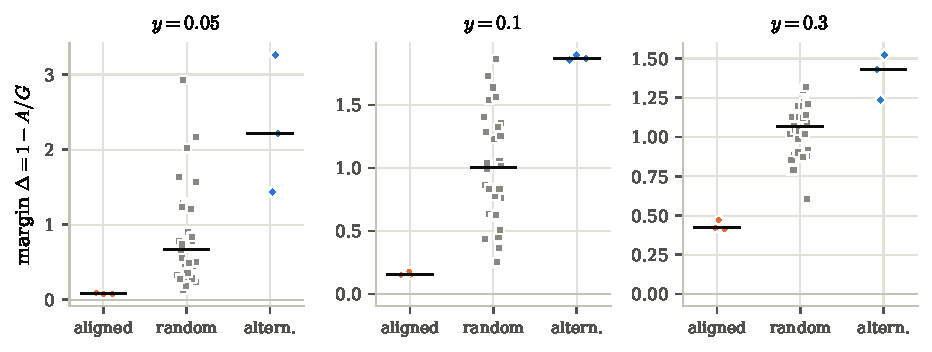
\includegraphics[width=0.95\textwidth]{fig5_margin_heights.pdf}
\caption{The margin $\Delta=1-A/G$ at the three best-aligned heights (circles), 30 random heights (squares) and the three best-alternating heights (diamonds) in $[2\times10^5,3.2\times10^6]$, at $y=0.05,0.1,0.3$. Bars mark medians. The aligned heights carry the three smallest margins at every $y$.}
\label{fig:heights}
\end{figure}

\paragraph{The margin.} At each of $y=0.05,0.1,0.3$ the medians are ordered, aligned $<$ random $<$ alternating: $0.078<0.670<2.214$, $0.155<1.003<1.866$ and $0.422<1.066<1.430$. Where the small-prime Euler factors align, the prime side is large and the margin small; where they alternate with the parity of $\Omega$, the prime side is negative: at the three alternating heights $\Delta>1$, that is $A<0$, at every $y$ in the table (\cref{fig:heights}). Among the $36$ heights, the three smallest margins at each $y$ occur at the aligned heights, exactly the heights at which the Wigner coefficients approach the unsigned divisor function. That large values of $|\zeta|$ and of $-\zeta'/\zeta$ occur at such heights is classical \cite[Ch.~VIII]{Titchmarsh}; what is measured here is the size of the effect on the margin of \eqref{eq:criterion}.

\section{The remaining step}\label{sec:target}
By \cref{prop:pairformula,prop:region}, $J>0$ on the whole upper half-plane outside $\mathcal U$, and RH is equivalent to $J\ge0$ on $\mathcal U$, that is, to Conjecture~\ref{conj:target}. The paper proves the following further equivalent forms of it:
\begin{enumerate}[label=(\alph*)]
\item every even position moment of the Wigner function of $\Phi$, at every momentum, is nonnegative (\cref{thm:moments});
\item $A\le G$ on $\mathcal U$, that is, the margin $\Delta$ is nonnegative there (\cref{prop:ledger});
\item $M(x)=O(x^{1/2+\varepsilon})$, equivalently $L(x)=O(x^{1/2+\varepsilon})$, for every $\varepsilon>0$: the balance of the sign pair (\cref{prop:RH});
\item every orbit of the mirror group $V_4$ on the nontrivial zeros has size $2$ (\cref{sec:eta});
\item the Riemann spin, the logarithm of the merged pair $Y$ weighted by $\sqrt Y$, is a Lee--Yang spin: $\frac12\int\Phi(u)e^{hu}\dd u$ vanishes only for imaginary $h$ (\cref{sec:horizon,sec:xi}; \cite{Newman74,Newman76,NewmanWu}); equivalently, a probe qubit dephased by a classical field with law $\Phi/2\Xi(0)$ has coherence $\Xi(\lambda t)/\Xi(0)$, and this coherence, continued to complex time, vanishes only at real $t$ \cite{SQuant}.
\end{enumerate}

\paragraph{What the paper fixes about the remaining step.} Positivity, evenness, doubly-exponential decay, the theta-series origin, an expansion of the form of \cref{thm:macdonald} and a tail theorem of the form of \cref{thm:tail} are shared by $\Phi_\epsilon$, whose current is negative near its off-line zero (\cref{rem:nogo}), and the mirror alone leaves the zeros of the Davenport--Heilbronn function off the line (\cref{sec:mirror}). A proof must use a property that these functions lack; the one this paper isolates is the merge, the Euler product. Kernel positivity alone reaches $y\gtrsim5.24x$ (\cref{cor:calib}); near the line the sign is decided in the oscillatory head, and at $x=50$ in the Airy transition zone (\cref{sec:ledger}); among the heights measured the margin is smallest where the coefficients approach $d(N)$ (\cref{sec:heights}). In the analytic form, the step is to control, uniformly in $x$, the transition-zone contribution to $\Num$ at heights where $\tau_x(N)$ approaches $d(N)$: a statement about Airy-regime sums of $d(N)K_{ix}(2\pi Ne^p)$.

In the spin form, the step is to carry the positive merge through the logarithm. A positive merge preserves the Lee--Yang property (\cref{prop:spin}); the merge in \cref{sec:xi} is additive, $S_2=S_1\oplus S_1'$, while the Riemann spin is its logarithm. One sufficient form is that $\Phi$ lies in the Griffiths--Simon class of limits of positively merged elementary pairs \cite{SimonGriffiths}; the Lee--Yang theorem then gives RH. Newman's theorem that $V'=-(\log\Phi)'$ is convex on $[0,\infty)$ is the first step towards it \cite{Newman91}; Newman writes the kernel in the variable $u/2$, which does not affect convexity. On the grid $u=0.01,0.02,\dots,3.00$, summing $\Phi$ over $n\le13$ and approximating $V'''$ by the central difference $[V(u+2h)-2V(u+h)+2V(u-h)-V(u-2h)]/2h^3$ with $h=10^{-7}$ in $60$-significant-digit decimal arithmetic, $V'''>0$ at every grid point and $\min V'''(u)/u=129.08$ (at $u=0.40$); exact term-by-term differentiation of the series in double precision gives the same values.

In the arithmetic form, the Selberg class is defined by axioms that include the mirror (a functional equation with gamma factors) and the merge (an Euler product), and the Selberg conjecture is that every member has its nontrivial zeros on the line \cite{Selberg}. The Davenport--Heilbronn function and $Z_\epsilon$ satisfy the mirror without the merge and have zeros off the line, so the merge axiom is essential. RH is the case of $\zeta$.

\paragraph{Where the merge stops.} The Euler product converges only for $\Re s>1$. The free prime gas of \cref{sec:merge} has a Hagedorn point at $\beta=1$, and a quantum statistical system with partition function $\zeta(\beta)$ has a phase transition there \cite{BostConnes}. The zeros lie beyond this point, in $0<\Re s<1$, where the merged representation is no longer a product. The first-zero path of \cref{sec:xi} shows this crossing for one zero: the prime-$2$ zero starts on $\Re s=1$ and is carried to the line by the merge. The unconditional results recalled in \cref{sec:intro}, the zero-free region near $\Re s=1$ \cite{MT}, the verification of RH to height $3\cdot10^{12}$ \cite{PT} and the proportions of \cref{tab:prop}, carry the balance part of the way.

\section{Methods of computation}\label{sec:methods}
This section states the numerical methods behind the computations of the paper, with their precision.

\paragraph{Arithmetic.} Two kinds of arithmetic are used. Double-precision computations use IEEE double precision (about 16 significant digits) and adaptive Gauss--Kronrod quadrature with relative tolerance $10^{-13}$. High-precision computations use decimal floating-point arithmetic with a fixed number of significant digits (40 to 200, stated at each use), with $\pi$ to more than 300 digits, $\exp$ and $\log$ to full working precision, $\cos$ and $\sin$ by their Taylor series after reduction modulo $2\pi$ (with ten guard digits), and $\cosh$ from $\exp$. The sieve of \cref{sec:balance} and the enumerations of \cref{sec:zero,sec:thirds} use exact integer and rational arithmetic.

\paragraph{Macdonald functions.} $K_{ix}(z)$ and $K'_{ix}(z)$ are computed simultaneously for $z=Nz_1$, $N=1,\dots,N_{\max}$, by the trapezoidal rule with step $h=2\pi/(2x+200)$ applied to $K_{ix}(z)=\int_0^We^{-z\cosh w}\cos(xw)\,dw$ and $-K'_{ix}(z)=\int_0^We^{-z\cosh w}\cosh w\cos(xw)\,dw$, where $W$ is chosen so that $e^{-z_1\cosh W}$ is below the working precision times $e^{-\pi x/2}$. The integrands are even and entire in $w$, so the trapezoidal error is aliasing-limited, of relative size about $\exp(-\frac\pi2(2\pi/h-2x))=e^{-100\pi}\approx10^{-136}$. Because $|K_{ix}(z)|$ is of order $e^{-\pi x/2}$ for $z<x$ while the integrand is of order $1$, the sum loses about $\pi x/(2\ln10)\approx0.68x$ digits to cancellation; this is why the working precision grows with $x$ ($60+0.7x$ digits in the scans of \cref{sec:positive}). For example, at 120 digits, changing the step from $2\pi/360$ to $2\pi/560$ or to $2\pi/720$ changes $K_{i\,80}(3)\approx1.3085673\times10^{-56}$ by a relative amount below $10^{-65}$, the precision left after the cancellation. The expansion of \cref{thm:macdonald} is truncated at $N_{\max}=\lfloor(x+P\ln10+40)/z_1\rfloor+2$ for $P$ working digits, beyond which the terms are below the working precision. In double precision, $K_{ix}$ and $K'_{ix}$ are computed by adaptive quadrature of the same integrals over $[0,\operatorname{arccosh}(1+745/z)]$. For rigorous bounds and algorithms for $K_{ix}$ see \cite{BST}.

\paragraph{The functions $\Xi$ and $\Xi_\epsilon$.} $\Xi(z)$, $\Xi'(z)$ and, on the real axis, $\Xi''(x)$ are computed from $\Xi(z)=\int_0^\infty\Phi(u)\cos(zu)\,du$ and its $z$-derivatives by the trapezoidal rule on $[0,3.5]$ with step $2\pi/(2\Re z+200)$, the series for $\Phi$ being truncated at $n\le14$ (the omitted terms are below $e^{-225\pi}$ relative to the first) and $\Phi(3.5)<\exp(-\pi e^7)$ being negligible. The integrand is even and analytic in a strip around the real axis, so the trapezoidal rule converges geometrically; the agreement of $J$ computed in this way with $J$ computed from $Q$ (\cref{sec:expansion}) to $2\times10^{-15}$ confirms this accuracy. $\Xi_\epsilon$ is computed in the same way from $\Phi_\epsilon$ (\cref{lem:epkernel}), keeping all terms with $a$ below $P\ln10+30$.

\paragraph{The zeta function and its relatives.} $\zeta(s)$ and $\zeta'(s)$ are computed in double precision by Euler--Maclaurin summation,
\[
\zeta(s)=\sum_{n<N}n^{-s}+\frac{N^{1-s}}{s-1}+\frac{N^{-s}}2+\sum_{k=1}^{M}\frac{B_{2k}}{(2k)!}\,s(s+1)\cdots(s+2k-2)\,N^{1-s-2k},
\]
and its term-by-term derivative, with $N=\max(200,|s|/\pi)+1$, $M=16$ or $20$, and the Bernoulli numbers $B_{2k}$ computed exactly as rationals. In the functional equation $\frac{\zeta'}\zeta(s)=\log2\pi+\frac\pi2\cot\frac{\pi s}2-\psi(1-s)-\frac{\zeta'}\zeta(1-s)$ the residual is $2.6\times10^{-13}$ at $s=0.55+50i$ and $8\times10^{-7}$ at $s=0.55+3.1\times10^6i$, where doubling $N$ changes $A=-\Re\zeta'/\zeta$ by $3\times10^{-8}$; the margins of \cref{sec:heights} are quoted to three decimals. At $s=2$ it gives $\zeta(2)=\pi^2/6$ to $2\times10^{-16}$ and $\zeta'/\zeta(2)=-0.5699609930945327$, whose numerator $\zeta'(2)$ agrees to $10^{-15}$ with direct summation of $-\sum_{n\le10^6}(\log n)/n^2$ plus its Euler--Maclaurin tail. For the computations of \cref{sec:eta} the same formula is used with the first $200$ terms and $16$ Bernoulli corrections, and the pair sums of $\eta$ by direct summation of $K$ pairs with the tail correction $\frac12(2K+1)^{-s}$. The completed values $\zeta^*(w)=\pi^{-w/2}\Gamma(\frac w2)\zeta(w)$ of \cref{prop:operator} use the same $\zeta$; the Gamma and digamma functions at complex argument are evaluated in double precision by recurrence and the Stirling series. The Hurwitz zeta values of \cref{sec:thirds,sec:mirror,sec:merge} are computed by the Euler--Maclaurin formula for $\zeta(s,\alpha)$ with $\lfloor|t|\rfloor+30$ terms and ten Bernoulli corrections, which reproduces the functional equation of $\zeta$ to a relative $1.5\times10^{-13}$ at heights up to $300$.

\section{Concluding remarks}\label{sec:concl}
We have written the Riemann Hypothesis as the positivity of a signed phase-space average of the Wigner function of Riemann's kernel, $J=\frac14\int Q\,p\sinh(yp)\,dp$; given the Wigner function an exact expansion in Macdonald functions with divisor-type coefficients and Mellin transform $8\,\xi(w+ix)\xi(w-ix)$; proved it positive beyond an explicit turning point at every momentum; and proved the current positive outside the set $\mathcal U$. The Epstein kernel of the form $2m^2+3n^2$ shares every property of Riemann's kernel used in these proofs except the Euler product of its coefficients, and its current is negative near its zero off the line. The Euler product is a merge: $\xi$ is the moment function of a merged pair, one copy carries the alternating series of the prime two, and the mirror of the functional equation holds only for the pair. The pair, the triad and the merge are exact statements about $\zeta$: the balance of the parity of $\Omega$, the thirds of $\mathbb Z/3$ and of the three-state spin, and the Lee--Yang property of positive merges.

\paragraph{Outlook.} The next step is Conjecture~\ref{conj:target} in its analytic form: uniform control of the Airy-regime sums of $d(N)K_{ix}(2\pi Ne^p)$ at the heights where $\tau_x(N)$ approaches $d(N)$, where the margin is smallest. In its spin form the step is to place $\Phi$ in the Griffiths--Simon class of positively merged elementary pairs, for which Newman's convexity theorem is the first step.

\section{Data and sources}\label{sec:data}
\paragraph{External numerical inputs.} All inputs are mathematical; no measured data are used.
\begin{enumerate}[label=(\roman*)]
\item All nontrivial zeros $\frac12+b+i\gamma$ of $\zeta$ with $0<\gamma\le3\cdot10^{12}$ have $b=0$ \cite{PT} (\cref{prop:region}).
\item $\zeta(\sigma+it)\ne0$ for $\sigma\ge1-1/(5.573412\log|t|)$, $|t|\ge2$, with the constant $5.573412$ \cite{MT} (\cref{prop:region}).
\item The ordinates of the first two zeros, $\gamma_1=14.134725141734693790\ldots$ and $\gamma_2=21.022039638771554993\ldots$, from Odlyzko's table of the first 100 zeros to over 1000 decimal places \cite{Odlyzko}, used to double precision as evaluation points (\cref{sec:current,sec:mellin,sec:eta}), in the evaluation of $\frac12\int\Phi(u)\cos(\gamma_1u)\dd u\approx0$ and as starting points of the zero paths of \cref{sec:xi}. Newton's method on $\Xi$ computed from the kernel integral in double precision reproduces them to $2\times10^{-12}$.
\item Spira's zeros of the Davenport--Heilbronn function, $0.808517+85.699348\,i$, $0.650830+114.163343\,i$, $0.574356+166.479306\,i$, $0.724258+176.702461\,i$ \cite{Spira}, used only for comparison (\cref{sec:mirror}).
\item Published values used for comparison: $M(10^k)$ for $k=1,\dots,8$: $-1,1,2,-23,-48,212,1037,1928$ (OEIS A084237 \cite{OEISM}); $L(10^k)$ for $k=1,\dots,8$: $0,-2,-14,-94,-288,-530,-842,-3884$ (OEIS A090410 \cite{OEISL}); the number of squarefree integers up to $10^8$, $60{,}792{,}694$ (OEIS A071172 \cite{OEISQ}). All agree with the computed values.
\item Published results quoted: the least $x\ge2$ with $L(x)>0$ is $906{,}150{,}257$ \cite{Tanaka}; $|M(x)|>\sqrt x$ for some $x$ \cite{OdlyzkoteRiele}; the proportion of nontrivial zeros proved to lie on the critical line exceeds $\frac13$ \cite{Levinson}, $\frac25$ \cite{Conrey} and $\frac5{12}$ \cite{PRZZ}, and a proportion at least $0.6725$, counted with multiplicity, is simple and on the line \cite{AF} (\cref{tab:prop}); the de Bruijn--Newman constant satisfies $\Lambda\ge0$ \cite{RT} and $\Lambda\le0.2$ \cite[Cor.~2]{PT} (\cref{sec:intro}).
\end{enumerate}

\paragraph{Computed quantities.} Every other number in the paper is computed from formulas stated in the text, by the methods of \cref{sec:methods}: $\Phi$, $\Xi$, $Q$, $K_{ix}$, $\tau_x(N)$ and the bounds of \cref{sec:euler,sec:positive}; $\xi(\frac12)=-\frac18\pi^{-1/4}\Gamma(\frac14)\zeta(\frac12)=0.4971207782$ with $\zeta(\frac12)=-1.4603545088$ from Euler--Maclaurin summation; $\zeta'/\zeta$, $G$, $A$ and $\Delta$; the Epstein kernel, $r_\epsilon(n)$ by enumeration of the solutions of $2m^2+3k^2=n$, and the zero $s_0$ (located by Newton's method on $\xi_\epsilon$, \cref{sec:epstein}); the aligned and alternating heights (by the searches of \cref{sec:heights}); $M(x)$, $L(x)$, the parity counts, the squarefree count and the grid values of \cref{fig:bal} (left), by the sieve of \cref{sec:balance} over all $n\le10^8$; the data for $\mathbb Z/n\mathbb Z$ ($n\le30$, and $n\le60$ in \cref{fig:bal}, right), by direct enumeration; the constant $\tan\vartheta$ from its closed form; the Davenport--Heilbronn and $L(s,\chi_{\pm})$ zero counts and the spin-chain zeros (\cref{sec:mirror,sec:merge}); and the moment functions, mirror ratios and zero paths of \cref{sec:xi}.

\paragraph{Heights of \cref{sec:heights}.} The aligned heights are the grid points of search (A) $2338770.254945$, $1671688.516551$, $2942100.234585$ (quoted to $10^{-3}$ in the text); the alternating heights are the grid points $2184674.890$, $1631971.391$, $706798.867$. The 30 random heights, drawn uniformly from $[2\times10^5,3.2\times10^6]$ at distance at least $100$ from the aligned heights, are, to $10^{-6}$:
\begin{center}\small
\begin{tabular}{@{}rrrrr@{}}
$397793.954544$ & $668910.133515$ & $2145087.674681$ & $1759893.950585$ & $325285.906206$\\
$2081053.108214$ & $1711897.090543$ & $2348615.979154$ & $892638.920828$ & $1220292.924432$\\
$1503280.458709$ & $2708229.558829$ & $711810.075210$ & $3039137.072760$ & $1442959.801814$\\
$2674176.500676$ & $2911059.367369$ & $1042432.414765$ & $684029.967108$ & $581987.254413$\\
$1048736.994616$ & $458182.890058$ & $1395206.686552$ & $626911.127533$ & $948534.574258$\\
$1819812.352119$ & $639981.006710$ & $572340.435135$ & $2886075.370007$ & $1856842.781951$\\
\end{tabular}
\end{center}

\paragraph{Contributions and use of AI.} The ideas, the research questions, the framework that links the fields, the choice of problems and the direction at every stage are the author's. The derivations, proofs, numerical checks, reference checks and drafting were produced with an AI system working under that direction, and were checked by separate AI review passes. Errors in that material are errors of the AI system, and any found will be corrected in a revised version. Publication-ethics policy (COPE, \emph{Authorship and AI tools}, 2023) does not allow an AI system to be listed as an author, so its use is declared here instead.

\begin{thebibliography}{99}\small
\bibitem{AF} L.~Alp\"oge, R.~Furman, More than two thirds of the zeros of the Riemann zeta function are simple and on the critical line, preprint, arXiv:2608.13637, 13 August 2026.
\bibitem{BerryKeating} M.~V.~Berry, J.~P.~Keating, The Riemann zeros and eigenvalue asymptotics, \emph{SIAM Rev.} 41 (1999) 236--266.
\bibitem{BGP} P.~Betzios, N.~Gaddam, O.~Papadoulaki, Black holes, quantum chaos, and the Riemann hypothesis, \emph{SciPost Phys. Core} 4 (2021) 032.
\bibitem{BPY} P.~Biane, J.~Pitman, M.~Yor, Probability laws related to the Jacobi theta and Riemann zeta functions, and Brownian excursions, \emph{Bull. Amer. Math. Soc.} 38 (2001) 435--465.
\bibitem{BST} A.~R.~Booker, A.~Str\"ombergsson, H.~Then, Bounds and algorithms for the $K$-Bessel function of imaginary order, \emph{LMS J. Comput. Math.} 16 (2013) 78--108.
\bibitem{Borwein} P.~Borwein, S.~Choi, B.~Rooney, A.~Weirathmueller (eds.), \emph{The Riemann Hypothesis: A Resource for the Afficionado and Virtuoso Alike}, CMS Books in Mathematics, Springer, New York, 2008.
\bibitem{BostConnes} J.-B.~Bost, A.~Connes, Hecke algebras, type III factors and phase transitions with spontaneous symmetry breaking in number theory, \emph{Selecta Math. (N.S.)} 1 (1995) 411--457.
\bibitem{Conrey} J.~B.~Conrey, More than two fifths of the zeros of the Riemann zeta function are on the critical line, \emph{J. Reine Angew. Math.} 399 (1989) 1--26.
\bibitem{CV} G.~Csordas, R.~S.~Varga, Necessary and sufficient conditions and the Riemann hypothesis, \emph{Adv. Appl. Math.} 11 (1990) 328--357.
\bibitem{DH} H.~Davenport, H.~Heilbronn, On the zeros of certain Dirichlet series I, II, \emph{J. London Math. Soc.} 11 (1936) 181--185, 307--312.
\bibitem{deBruijn} N.~G.~de Bruijn, The roots of trigonometric integrals, \emph{Duke Math. J.} 17 (1950) 197--226.
\bibitem{Dunster} T.~M.~Dunster, Bessel functions of purely imaginary order, with an application to second-order linear differential equations having a large parameter, \emph{SIAM J. Math. Anal.} 21 (1990) 995--1018.
\bibitem{Griffiths69} R.~B.~Griffiths, Rigorous results for Ising ferromagnets of arbitrary spin, \emph{J. Math. Phys.} 10 (1969) 1559--1565.
\bibitem{HardyWright} G.~H.~Hardy, E.~M.~Wright, \emph{An Introduction to the Theory of Numbers}, 6th ed., revised by D.~R.~Heath-Brown and J.~H.~Silverman, Oxford University Press, Oxford, 2008.
\bibitem{Haselgrove} C.~B.~Haselgrove, A disproof of a conjecture of P\'olya, \emph{Mathematika} 5 (1958) 141--145.
\bibitem{Hudson} R.~L.~Hudson, When is the Wigner quasi-probability density non-negative?, \emph{Rep. Math. Phys.} 6 (1974) 249--252.
\bibitem{Iwaniec} H.~Iwaniec, \emph{Spectral Methods of Automorphic Forms}, 2nd ed., Graduate Studies in Mathematics 53, American Mathematical Society, Providence, RI, 2002.
\bibitem{Lagarias} J.~C.~Lagarias, On a positivity property of the Riemann $\xi$-function, \emph{Acta Arith.} 89 (1999) 217--234; correction, \emph{Acta Arith.} 116 (2005) 293--294.
\bibitem{Lang} S.~Lang, \emph{Algebra}, 3rd ed., Graduate Texts in Mathematics 211, Springer, New York, 2002.
\bibitem{LeeYang} T.~D.~Lee, C.~N.~Yang, Statistical theory of equations of state and phase transitions. II. Lattice gas and Ising model, \emph{Phys. Rev.} 87 (1952) 410--419.
\bibitem{Levinson} N.~Levinson, More than one third of zeros of Riemann's zeta-function are on $\sigma=1/2$, \emph{Adv. Math.} 13 (1974) 383--436.
\bibitem{Littlewood} J.~E.~Littlewood, Quelques cons\'equences de l'hypoth\`ese que la fonction $\zeta(s)$ de Riemann n'a pas de z\'eros dans le demi-plan $\Re(s)>\frac12$, \emph{C. R. Acad. Sci. Paris} 154 (1912) 263--266.
\bibitem{MT} M.~J.~Mossinghoff, T.~S.~Trudgian, Nonnegative trigonometric polynomials and a zero-free region for the Riemann zeta-function, \emph{J. Number Theory} 157 (2015) 329--349.
\bibitem{Newman74} C.~M.~Newman, Zeros of the partition function for generalized Ising systems, \emph{Comm. Pure Appl. Math.} 27 (1974) 143--159.
\bibitem{Newman76} C.~M.~Newman, Fourier transforms with only real zeros, \emph{Proc. Amer. Math. Soc.} 61 (1976) 245--251.
\bibitem{Newman91} C.~M.~Newman, The GHS inequality and the Riemann hypothesis, \emph{Constr. Approx.} 7 (1991) 389--399.
\bibitem{NewmanWu} C.~M.~Newman, W.~Wu, Constants of de Bruijn--Newman type in analytic number theory and statistical physics, \emph{Bull. Amer. Math. Soc.} 57 (2020) 595--614.
\bibitem{DLMF} NIST Digital Library of Mathematical Functions, \S\S10.32, 10.40, 10.43, \url{https://dlmf.nist.gov} (accessed 24 September 2026).
\bibitem{Odlyzko} A.~M.~Odlyzko, Tables of zeros of the Riemann zeta function, \url{https://www-users.cse.umn.edu/~odlyzko/zeta_tables/index.html} (accessed 24 September 2026).
\bibitem{OdlyzkoteRiele} A.~M.~Odlyzko, H.~J.~J.~te Riele, Disproof of the Mertens conjecture, \emph{J. Reine Angew. Math.} 357 (1985) 138--160.
\bibitem{OEISQ} OEIS Foundation, Sequence A071172, number of squarefree integers $\le10^n$, \emph{The On-Line Encyclopedia of Integer Sequences}, \url{https://oeis.org/A071172} (accessed 24 September 2026).
\bibitem{OEISM} OEIS Foundation, Sequence A084237, $a(n)=M(10^n)$, where $M(n)$ is Mertens's function, \emph{The On-Line Encyclopedia of Integer Sequences}, \url{https://oeis.org/A084237} (accessed 24 September 2026).
\bibitem{OEISL} OEIS Foundation, Sequence A090410, values of $L(10^n)$, where $L(n)$ is the summatory function of the Liouville function, \emph{The On-Line Encyclopedia of Integer Sequences}, \url{https://oeis.org/A090410} (accessed 24 September 2026).
\bibitem{Patrick} M.~L.~Patrick, Extensions of inequalities of the Laguerre and Tur\'an type, \emph{Pacific J. Math.} 44 (1973) 675--682.
\bibitem{PT} D.~Platt, T.~Trudgian, The Riemann hypothesis is true up to $3\cdot10^{12}$, \emph{Bull. London Math. Soc.} 53 (2021) 792--797.
\bibitem{PRZZ} K.~Pratt, N.~Robles, A.~Zaharescu, D.~Zeindler, More than five-twelfths of the zeros of $\zeta$ are on the critical line, \emph{Res. Math. Sci.} 7 (2020) 2.
\bibitem{RT} B.~Rodgers, T.~Tao, The de Bruijn--Newman constant is non-negative, \emph{Forum Math. Pi} 8 (2020) e6.
\bibitem{Rota} G.-C.~Rota, On the foundations of combinatorial theory I: theory of M\"obius functions, \emph{Z. Wahrscheinlichkeitstheorie verw. Gebiete} 2 (1964) 340--368.
\bibitem{Selberg} A.~Selberg, Old and new conjectures and results about a class of Dirichlet series, in \emph{Proceedings of the Amalfi Conference on Analytic Number Theory} (1989), Univ. Salerno, Salerno, 1992, 367--385.
\bibitem{Sierra} G.~Sierra, The Riemann zeros as energy levels of a Dirac fermion in a potential built from the prime numbers in Rindler spacetime, \emph{J. Phys. A} 47 (2014) 325204.
\bibitem{SimonGriffiths} B.~Simon, R.~B.~Griffiths, The $(\phi^4)_2$ field theory as a classical Ising model, \emph{Commun. Math. Phys.} 33 (1973) 145--164.
\bibitem{SQuant} A.~Singh, The Riemann Kernel as a Quantum State: Wigner Negativity, Decoherence at the Thirds and Lee--Yang Zeros, manuscript, 25 September 2026.
\bibitem{SAlg} A.~Singh, Three Is Enough: Radix Economy, Balanced-Ternary Arithmetic and Ternary-Weight Networks, manuscript, 25 September 2026.
\bibitem{SSynth} A.~Singh, What a Zero Is: One Involution across Mathematics, Physics, Chemistry, Neuroscience, Computation and the Giant Planets, manuscript, 25 September 2026.
\bibitem{SD} J.~Sondow, C.~Dumitrescu, A monotonicity property of Riemann's xi function and a reformulation of the Riemann hypothesis, \emph{Period. Math. Hungar.} 60 (2010) 37--40.
\bibitem{Spector} D.~Spector, Supersymmetry and the M\"obius inversion function, \emph{Commun. Math. Phys.} 127 (1990) 239--252.
\bibitem{Spira} R.~Spira, Some zeros of the Titchmarsh counterexample, \emph{Math. Comp.} 63 (1994) 747--748.
\bibitem{Takagi} S.~Takagi, Vacuum noise and stress induced by uniform acceleration: Hawking--Unruh effect in Rindler manifold of arbitrary dimension, \emph{Prog. Theor. Phys. Suppl.} 88 (1986) 1--142.
\bibitem{Tanaka} M.~Tanaka, A numerical investigation on cumulative sum of the Liouville function, \emph{Tokyo J. Math.} 3 (1980) 187--189.
\bibitem{Titchmarsh} E.~C.~Titchmarsh, \emph{The Theory of the Riemann Zeta-Function}, 2nd ed., revised by D.~R.~Heath-Brown, Oxford University Press, Oxford, 1986.
\bibitem{Unruh} W.~G.~Unruh, Notes on black-hole evaporation, \emph{Phys. Rev. D} 14 (1976) 870--892.
\end{thebibliography}
\end{document}
